\documentclass[12pt,a4paper]{article}

\usepackage[english,italian]{babel}
\usepackage[utf8]{inputenc}
\usepackage{hyperref} 
\hypersetup{
    bookmarks=true,         % show bookmarks bar?
    % unicode=false,          % non-Latin characters in Acrobat’s bookmarks
    % pdftoolbar=true,        % show Acrobat’s toolbar?
    pdfmenubar=true,        % show Acrobat’s menu?
    % pdffitwindow=false,     % window fit to page when opened
    pdfstartview={FitH},    % fits the width of the page to the window
    pdftitle={Note di Algoritmi},    % title
    pdfauthor={Timoty Granziero},     % author
    % pdfsubject={},   % subject of the document 
    % pdfcreator={Creator},   % creator of the document
    % pdfproducer={Producer}, % producer of the document
    % pdfkeywords={keyword1, key2, key3}, % list of keywords
    % pdfnewwindow=true,      % links in new PDF window
    colorlinks=true,       % false: boxed links; true: colored links
    linkcolor=black,          % color of internal links (change box color with linkbordercolor)
    % citecolor=green,        % color of links to bibliography
    % filecolor=magenta,      % color of file links
    urlcolor=cyan           % color of external links
}

\usepackage{graphicx} %img/media
\usepackage{xcolor} %colors

\usepackage{enumitem} %lists
\usepackage[perpage]{footmisc} %footnote, starting at 1 every page

\usepackage{mathtools,stmaryrd} %math package
\usepackage{amssymb} % N, R ... symbols

\usepackage{totpages} % Per totale pagine

% per frecce in tutte le direzioni, comando \arrow{0}, \arrow{1}, etc.. 
\makeatletter
\newcommand{\fixed@sra}{$\vrule height 2\fontdimen22\textfont2 width 0pt\rightarrow$}
\newcommand{\arrow}[1]{%
  \mathrel{\text{\rotatebox[origin=c]{\numexpr#1*45}{\fixed@sra}}}
}
\makeatother

\usepackage{cancel}
\usepackage{appendix}

\let\emph\relax % there's no \RedeclareTextFontCommand
\DeclareTextFontCommand{\emph}{\bfseries} %emph to textbf

%floor and ceil
\DeclarePairedDelimiter\ceil{\lceil}{\rceil}
\DeclarePairedDelimiter\floor{\lfloor}{\rfloor}

%abs and norm
\DeclarePairedDelimiter\abs{\lvert}{\rvert}%
\DeclarePairedDelimiter\norm{\lVert}{\rVert}%

% Swap the definition of \abs* and \norm*, so that \abs
% and \norm resizes the size of the brackets, and the 
% starred version does not.
\makeatletter
\let\oldabs\abs
\def\abs{\@ifstar{\oldabs}{\oldabs*}}
%
\let\oldnorm\norm
\def\norm{\@ifstar{\oldnorm}{\oldnorm*}}
\makeatother

\usepackage{clrscode3e} % algorithms pseudocode
\RequirePackage{graphics} % needed for \scalebox command

\usepackage{tikz-qtree} %trees

\newcommand{\authorName}{Timoty Granziero}

%prevent page break
\newenvironment{preventpagebreak}
{\par\nobreak\vfil\penalty0\vfilneg
	\vtop\bgroup}
{\par\xdef\tpd{\the\prevdepth}\egroup
	\prevdepth=\tpd}

%liste
\renewcommand{\labelitemi}{$\circ$}
\renewcommand{\labelitemii}{$\cdot$}
\renewcommand{\labelitemiii}{$\diamond$}
\renewcommand{\labelitemiv}{$\ast$}

% add spacing after exists and forall
\let\existstemp\exists
\let\foralltemp\forall
\renewcommand{\exists}{\existstemp~}
\renewcommand{\forall}{\foralltemp~}

\author{\authorName}
\date{\today}
\title{Appunti di Algoritmi}


\usepackage{fancyhdr} %header e footer

%header/footer setup
\fancyhf{}
\fancyhead[R]{\small\scshape\nouppercase{\leftmark}}
\fancyhead[L]{\small\scshape\nouppercase{\rightmark}}
%\fancyhead[L,R]{\small\thepage}
\lhead{\nouppercase{\rightmark}}
\rhead{\nouppercase{\leftmark}}
\cfoot{\thepage}
%\lfoot{\authorName}

\pagestyle{fancy}


% \includeonly{rel/lez_04_27}

\begin{document} 

\begin{titlepage} 
	\centering
	
\includegraphics[width=0.50\textwidth]{img/logo.pdf}\par\vspace{1cm} %logo
	
	{\LARGE\bfseries Appunti di Algoritmi e Strutture Dati \par}
	\vspace{1cm}
	
	{\Large\bfseries a.a. 2017/2018 \par}
	
	\vspace{1cm} 

	Autore: \par
	{\bfseries \authorName \par} 
	
	\vspace{1cm}

	Repository: \par
	\url{https://github.com/Vashy/ASD-Notes}
    
    \vfill
	
	% Bottom of the page
	{\large \today\par}
	
\end{titlepage}

\tikzset{every tree node/.style={minimum width=2em,draw,circle},
	blank/.style={draw=none},
	edge from parent/.style=
	{draw,edge from parent path={(\tikzparentnode) -- (\tikzchildnode)}},
	level distance=1.5cm}

\newpage
\tableofcontents

\frenchspacing

\section{Lezione del 28/02/2018}

\subsection{Problem Solving}
\begin{enumerate}
	\item Formalizzazione del problema;
	\item Sviluppo dell'\textbf{algoritmo} (focus del corso);
	\item Implementazione in un programma (codice).
\end{enumerate}

\paragraph{Algoritmo} Sequenza di passi elementari che risolve il problema.\par

\begin{center}
	Input $\rightarrow$ \textbf{Algoritmo} $\rightarrow$ Output
\end{center}

\begin{quote} 
	\textit{Dato un problema, ci sono tanti algoritmi per risolverlo.}
\end{quote}

\noindent \textbf{e.g.}\footnote{For the sake of example.} Ordinamento dei numeri di una \texttt{Rubrica}.
L'idea è quella di trovare tutte le permutazioni di ogni numero.\par
\begin{gather*}
	\text{30 numeri: \textit{complessità} } 30! \cong 2 \times 10^{32}ns \Rightarrow \\
	3^{19} \text{anni (con \textit{ns} = nanosecondi)}
\end{gather*}

\paragraph{std::vector} È un esempio nel \texttt{C++} delle ragioni per cui 
si studia questa materia. Nella documentazione della \texttt{STL}, 
sono riportati i seguenti:

\begin{itemize}
	\item \texttt{Random access}: complessità $O(1)$;
	\item \texttt{Insert}: complessità $O(1)$ ammortizzato.
\end{itemize}

Il \texttt{random access} è l'accesso a un elemento casuale del \texttt{vector}. 
$O(1)$ implica che l'accesso avviene in tempo costante (pari a 1). \par
Per \texttt{insert} si intende l'inserimento di un nuovo elemento in coda. 
Avviene in tempo $O(1)$ ammortizzato: questo perchè ogni N inserimenti, è 
necessario un resize del vector e una copia di tutti gli elementi nel nuovo vettore
(questa procedura è nascosta al programmatore).

\subsection{Cosa analizzeremo nel corso}

\begin{itemize}
	\item[$\bullet$] Tempo di esecuzione;
	\item[$\bullet$] Spazio (memoria);
	\medskip
	\item Correttezza;
	\item Manutenibilità.
\end{itemize}

\subsubsection{Approfondimento sul tempo di esecuzione T(n)}

\begin{itemize}
	\item \textit{P Problems}: complessità polinomiale. L'algoritmo è trattabile
	\item \textit{NP Complete}: problemi NP completi. \textbf{e.g}: Applicazione sugli algoritmi di sicurezzza. Si basano sull'assunzione che per essere risolti debbano essere considerate tutte le soluzioni possibili.
	\item \textit{NP Problems}: problemi con complessità  (ad esempio) esponenziale/ fattoriale. Assolutamente non trattabili.
\end{itemize}

\begin{figure}[htb]
	\centering
	\includegraphics[height=6cm]{img/algorithm_complexity.png}
	\caption{Complessità T(n).}	
\end{figure}
	
\subsection{Problema dell'ordinamento (sorting)}
\texttt{Input}: sequenza di numeri 
\begin{center}
	$a_0 a_1 \dots a_n$;\par
\end{center}
\texttt{Output}: permutazione
\begin{center}
	$a'_0 a'_1 \dots a'_n$
\end{center}
tale che 
\begin{center}
	$a'_0 \leq a'_1 \leq \dots \leq a'_n$
\end{center}

\noindent Vedremo due algoritmi:
\begin{itemize}[noitemsep]
	\item \texttt{Insertion Sort};
	\item \texttt{Merge Sort}.
\end{itemize}

\subsection{Insertion Sort} \label{insertionsort}
\href{https://en.wikipedia.org/wiki/Insertion_sort}{Insertion Sort} un algoritmo di \emph{sorting incrementale}. Viene applicato naturalmente ad esempio quando si vogliono ordinare le carte nella propria mano in una partita a scala 40: si prende ogni carta a partire da sinistra, e la si posiziona in ordine crescente.\par
\paragraph{Astrazione} Prendiamo ad esempio il seguente array:

\begin{center}
	\begin{tabular}{|l|l|l|l|l|}
		\hline
		5 & 2 & 8 & 4 & 7 \\
		\hline
	\end{tabular}
\end{center}

\noindent Partiamo dal primo elemento: 5. È già ordinato con se stesso, quindi procediamo con il secondo elemento.\par
\noindent Confronto il numero 2 con l'elemento alla sua sinistra: \par
$2 \geq 5$?  No, quindi lo inverto con l'elemento alla sua sinistra, come segue

\begin{center}
	\begin{tabular}{|l|l|l|l|l|}
		\hline
		2 & 5 & 8 & 4 & 7 \\
		\hline
	\end{tabular}
	\hspace{1cm} Key: 
	\begin{tabular}{|l|}
		\hline
		8 \\
		\hline
	\end{tabular}
\end{center}

\noindent La key analizzata è 8. \par
$8 \geq 5$? Sì, quindi è ordinato in modo corretto.

\begin{center}
	\begin{tabular}{|l|l|l|l|l|}
		\hline
		2 & 5 & 8 & 4 & 7 \\
		\hline
	\end{tabular}
	\hspace{1cm} Key: 
	\begin{tabular}{|l|}
		\hline
		4 \\
		\hline
	\end{tabular}
\end{center}

\noindent La key analizzata è 4.\par
$4 \geq 8$? No, quindi lo sposto a sinistra invertendolo con 8.\par 
$4 \geq 5$? No, lo sposto a sinistra invertendolo con 5.\par
$4 \geq 2$? Sì, quindi è nella posizione corretta.

\begin{center}
	\begin{tabular}{|l|l|l|l|l|}
		\hline
		2 & 4 & 5 & 8 & 7 \\
		\hline
	\end{tabular}
	\hspace{1cm} Key: 
	\begin{tabular}{|l|}
		\hline
		7 \\
		\hline
	\end{tabular}
\end{center}

\noindent Key analizzata 7. \par
$7 \geq 8$? No, lo sposto a sinistra invertendolo con 8.\par
$7 \geq 5$? Sì, è nella posizione corretta.\par

\smallskip
\noindent Ottengo l'array ordinato:

\begin{center}
	\begin{tabular}{|l|l|l|l|l|}
		\hline
		2 & 4 & 5 & 7 & 8 \\
		\hline
	\end{tabular}
\end{center}

\newpage

\paragraph{Algorimo} Passiamo ora all'implementazione dell'algoritmo, con uno pseudocodice similare a \texttt{Python}\footnote{\textbf{ATTENZIONE}: verranno usati array con indici
che partono da 1.}\par

\bigskip

\texttt{Input}: $A[1, \twodots ,n]$, $A.length$.

\begin{center}
	È noto che: 
	$A[i] \leq key < A[i+1]$
\end{center}

\paragraph{Pseudocodice} Segue lo pseudocodice dell'\texttt{Insertion Sort}.

\begin{codebox}
\Procname{\proc{InsertionSort}$(A)$}
\li $n \gets \attrib{A}{length}$
\li \For $j \gets 2$ \To $n$
	\Comment il primo elemento è già ordinato
\li		\Do
			$\id{key} \gets A[j]$ 
			\Comment $A[1 \twodots j-1]$ ordinato
\li			$i \gets j-1$
\li			\While $i > 0$ and $A[i] > \id{key}$
\li				\Do
					$A[i+1] \gets A[i]$
\li					$i \gets i-1$
				\End
\li			$A[i+1] \gets \id{key}$
		\End
\end{codebox}

\vspace{0.5cm}

Quando il \texttt{while} termina, ci sono due casi: 
\begin{itemize}
	\item[$\circ$] \texttt{i = 0}: tutti gli elementi prima di \texttt{j} 
	sono maggiori di \texttt{key}; \texttt{key} va al primo posto (1);
	\item[$\circ$] \texttt{(i > 0) and (A[i] $\leq$ key)}: \texttt{A[i+1] = key}.
\end{itemize}

\subsubsection{Invarianti e correttezza}

\paragraph{for} \texttt{A[1$\twodots$j-1]} è ordinato e contiene gli 
elementi in \texttt{(1,j-1)} iniziali.

\paragraph{while} \texttt{A[1$\twodots$i]A[i+2$\twodots$j]} ordinato e 
\texttt{A[i+2$\twodots$j] > key}. \par
\vspace{0.5cm}
In uscita abbiamo: 
\begin{itemize}[noitemsep]
	\item[$\circ$] \texttt{j = n+1}; \par
	\item[$\circ$] \texttt{A[1$\twodots$n]} ordinato, come da invariante: 
	vale \texttt{A[1$\twodots$j-1]}	ordinato, e \texttt{j} vale \texttt{n+1}.
\end{itemize} 

\section{Lezione del 02/03/2018}

\subsection{Modello dei costi}
\paragraph{Assunzione} Tutte le istruzioni richiedono un tempo \underline{costante}.

Rivediamo l'algoritmo:

\begin{codebox}
\Procname{\proc{InsertionSort}$(A)$}
\li $n \gets \attrib{A}{length}$
\li \For $j \gets 2$ \To $n$
	\Comment il primo elemento è già ordinato
\li		\Do
			$\id{key} \gets A[j]$ 
			\Comment $A[1 \twodots j-1]$ ordinato
\li			$i \gets j-1$
\li			\While $i > 0$ and $A[i] > \id{key}$
\li				\Do
					$A[i+1] \gets A[i]$
\li					$i \gets i-1$
				\End
\li			$A[i+1] \gets \id{key}$
		\End
\end{codebox}

Diamo il nome $c_0$ alla chiamata del metodo, \texttt{InsertionSort(A)};
A ogni riga numerata, diamo il nome $c_1, c_2,\twodots ,c_8$
\footnote{($c_1$ corrisponde alla riga 1, $c_2$ alla riga 2 e così via).}.\par
Vediamo il \emph{costo} di ogni istruzione:

\begin{itemize}
    \item[] $\boldsymbol{c_0} \rightarrow 1$
    \item[] $\boldsymbol{c_1} \rightarrow 1$
    \item[] $\boldsymbol{c_2} \rightarrow n$
    \item[] $\boldsymbol{c_3} \rightarrow (n-1)$
    \item[] $\boldsymbol{c_4} \rightarrow (n-1)$
    \item[] $\boldsymbol{c_5} \rightarrow \displaystyle\sum_{j=2}^{n} t_j+1$
    \item[] $\boldsymbol{c_6}, \boldsymbol{c_7} \rightarrow \displaystyle\sum_{j=2}^{n} t_j$
    \item[] $\boldsymbol{c_8} \rightarrow (n-1)$
\end{itemize}

\subsection{Complessità di IS} \label{is:complessita}
\begin{displaymath}
    T^{IS}(n) = c_0 + c_1 + c_2n + (c_3+c_4+c_8)(n-1)
    + c_5\displaystyle\sum_{j=2}^{n}(t_j+1) + (c_6+c_7)\displaystyle\sum_{j=2}^{n}t_j
\end{displaymath}

$\boldsymbol{t_j}$ dipende, oltre che da $n$, dall'istanza dell'array
che stiamo considerando.
È chiaro che questo calcolo non da indicazioni precise sull'effettiva
complessità dell'algoritmo.\par

\bigskip
Andiamo ad analizzare i 3 possibili casi:

\begin{enumerate}[label=\emph{\alph*})]
    \item Caso migliore (\ref{is:casomigliore})
    \item Caso peggiore (\ref{is:casopeggiore})
    \item Caso medio (\ref{is:casomedio})
\end{enumerate}

\subsubsection{Caso migliore} \label{is:casomigliore}

$\rightarrow A$ ordinato $\Rightarrow t_j = 0 $ $\forall j$

\bigskip
La \textbf{complessità} diventa:
\begin{displaymath}
    T^{IS}_{min}(n) = c_0 + c_1 + c_2n + (c_3+c_4+c_5+c_8)(n-1) 
    = an+b \approx n
\end{displaymath}

Ossia, si comporta come $n$. Il \emph{caso migliore} \textbf{non}
è interessante, visto che è improbabile si presenti.

\subsubsection{Caso peggiore} \label{is:casopeggiore}

$\rightarrow A$ ordinato in senso inverso $\Rightarrow \forall j$ $t_j = j-1$ \par
\bigskip
La \textbf{complessità} diventa: 

\begin{displaymath}
    T^{IS}_{max}(n) = c_0 + c_1 + c_2n + (c_3+c_4+c_8)(n-1)
    + c_5\displaystyle\sum_{j=2}^{n}j + (c_6+c_7)
    \displaystyle\sum_{j=2}^{n}(j-1)
\end{displaymath}

Per valutare il costo di $\displaystyle\sum_{j=2}^{n}j$ e di 
$\displaystyle\sum_{j=2}^{n}(j-1)$, usiamo la \textbf{somma di Gauss}: \par

\begin{equation}
    \displaystyle\sum_{i=1}^{n}i = \frac{n(n+1)}{2}
\end{equation}
\newpage
Otteniamo:

\begin{displaymath}
    \displaystyle\sum_{j=2}^{n}j = \frac{n(n+1)}{2}-1
\end{displaymath}

\begin{displaymath}
    \displaystyle\sum_{j=2}^{n}(j-1) = \displaystyle\sum_{i=1}^{n}n = \frac{(n-1)n}{2}
\end{displaymath}

Per finire, ricalcoliamo $T^{IS}_{max}(n)$

\begin{displaymath}
    T^{IS}_{max}(n) = a'n^2+b'n+c' \approx n^2
\end{displaymath}

\subsubsection{Caso medio} \label{is:casomedio}
Il caso medio è \emph{difficile da calcolare}, e in una considerevole parte dei casi,
coincide con il caso peggiore.\par
Comunque, l'idea è la seguente:

\begin{align*}
    \frac{\displaystyle\sum_{\text{perm. di input}}T^{IS}(p)}{n!} \approx n^2 && 
        \text{posso pensare che } t_j \cong \frac{j-1}{2}
\end{align*}

\subsection{Divide et Impera}

Un algoritmo di sorting \emph{divide et impera} si può suddividere in 3 fasi:

\begin{description}
    \item[divide] divide il problema dato in sottoproblemi più piccoli;
    \item[impera] risolve i sottoproblemi:
    \begin{itemize}
        \item ricorsivamente;
        \item la soluzione è nota (e.g. array con un elemento);
    \end{itemize}
    \item[combina] compone le soluzioni dei sottoproblemi in una soluzione del 
        problema originale.
\end{description}

\subsection{Merge Sort} \label{mergesort}
\href{https://en.wikipedia.org/wiki/Merge_sort}{Merge Sort}\footnote{Si %
consiglia di dare uno sguardo all'algoritmo anche da altre fonti, poichè presentarlo %
graficamente in \LaTeX, come è stato visto a lezione, non è facile.} è un 
esempio di algoritmo \emph{divide et impera}. Andiamo ad analizzarlo.

\paragraph{Astrazione} Consideriamo il seguente array A.
\begin{center}
	\begin{tabular}{|l|l|l|l||l|l|l|l|}
		\hline
		5 & 2 & 4 & 7 & 1 & 2 & 3 & 6 \\
		\hline
	\end{tabular}
\end{center}

Lo divido a metà, ottenendo due parti separate.

\begin{center}
	\begin{tabular}{|l|l|l|l|}
		\hline
		5 & 2 & 4 & 7 \\
		\hline
	\end{tabular}
	\hspace{1cm}
	\begin{tabular}{|l|l|l|l|}
		\hline
		1 & 2 & 3 & 6 \\
		\hline
	\end{tabular}
\end{center}

Consideriamo il primo, ossia \texttt{A[1$\twodots$4]} (A originale). Divido anche questo a metà.

\begin{center}
	\begin{tabular}{|l|l|}
		\hline
		5 & 2 \\
		\hline
	\end{tabular}
	\hspace{1cm}
	\begin{tabular}{|l|l|}
		\hline
		4 & 7 \\
		\hline
	\end{tabular}
\end{center}

Divido nuovamente a metà, ottenendo:

\begin{center}
	\begin{tabular}{|l|}
		\hline
		5 \\
		\hline
	\end{tabular}
	\hspace{1cm}
	\begin{tabular}{|l|}
		\hline
		2 \\
		\hline
	\end{tabular}
\end{center}

5 e 2 sono due blocchi già ordinati. Scelgo il minore tra i due e lo metto in prima 
posizione, mentre l'altro in seconda posizione, ottenendo un blocco composto da 2 e 5.\par
Riprendo con il blocco composto da 4 e 7. Lo divido in due blocchi da un elemento. Faccio lo stesso procedimento 
fatto per 2 e 5: metto in prima posizione 4 e in seconda posizione 7. La situazione
è la seguente:

\begin{center}
	\begin{tabular}{|l|l|}
		\hline
		2 & 5 \\
		\hline
	\end{tabular}
	\hspace{1cm}
	\begin{tabular}{|l|l|}
		\hline
		4 & 7 \\
		\hline
	\end{tabular}
\end{center}

So che i blocchi ottenuti contengono elementi ordinati. Con questa assunzione, posso ragionare 
nel seguente modo: considero il primo elemento dei due blocchi (2 e 4 in questo caso) e metto 
in prima posizione il minore tra i due. Ora considero il successivo elemento del blocco che è stato scelto e lo stesso elemento dell'altro blocco, e inserisco nell'array l'elemento minore. Continuo fino ad 
ottenere un blocco ordinato.

\begin{center}
	\begin{tabular}{|l|l|l|l|}
		\hline
		2 & 4 & 5 & 7 \\
		\hline
	\end{tabular}
\end{center}

Faccio lo stesso procedimento con la parte di array originale \texttt{A[5$\twodots$8]}, ottenendo

\begin{center}
	\begin{tabular}{|l|l|l|l|}
		\hline
		2 & 4 & 5 & 7 \\
		\hline
	\end{tabular}
	\hspace{1cm}
	\begin{tabular}{|l|l|l|l|}
		\hline
		1 & 2 & 3 & 6 \\
		\hline
	\end{tabular}
\end{center}

A questo punto, i blocchi da 4 contengono elementi tra loro ordinati. Faccio lo stesso ragionamento
usato per comporli, per ottenere l'array originale ordinato. Considero\footnote{Questo procedimento è stato applicato %
anche ai passaggi precedenti; qui è spiegato più rigorosamente.}:
\begin{itemize}[noitemsep]
    \item \texttt{L[1$\twodots$4] $=$ A[1$\twodots$4]}: indice $i = 1$ per scorrerlo;
    \item \texttt{R[1$\twodots$4] $=$ A[5$\twodots$8]}: indice $j = 1$ per scorrerlo;
\end{itemize}

Valuto \texttt{L[i]} e \texttt{R[j]}. \par
\begin{itemize}[noitemsep]
    \item Se \texttt{L[i]} $\leq$ \texttt{R[j]}, inserisco \texttt{L[i]} e incremento \texttt{i}. \par
    \item Altrimenti, inserisco \texttt{R[j]} e incremento \texttt{j}.
    \item Itero finchè entrambi gli indici non sono out of bounds.
\end{itemize}

\paragraph{Pseudocodice} Segue lo pseudocodice del 
\texttt{Merge Sort}.

\begin{codebox}
\Procname{\proc{MergeSort}$(A,p,r)$}
\li \If $p < r$
\li     \Then
            $q \gets \floor{\frac{p + r}{2}}$ 
        \Comment arrotondato per difetto
\li         $\proc{MergeSort}(A,p,q)$
        \Comment ordina \texttt{A[p$\twodots$q]}
\li         $\proc{MergeSort}(A,q+1,r)$
        \Comment ordina \texttt{A[q+1$\twodots$r]}
\li         $\proc{Merge}(A,p,q,r)$
        \Comment ``Merge'' dei due sotto-array 
        \End
\end{codebox}

\begin{codebox}
\Procname{\proc{Merge}$(A,p,q,r)$}
\li $\id{n1} \gets q-p+1$
    \Comment gli indici partono da 1
\li $\id{n2} \gets r-q$
\zi \Comment \kw{L} sotto-array sx, \kw{R} sotto-array dx
\li \For $i \gets 1$ \To $\id{n1}$
\li     \Do
            $L[i] \gets A[p+i-1]$
        \End
\li	\For $j \gets 1$ \To $\id{n2}$
\li		\Do
			$R[j] \gets A[q+j]$
        \End
\li         $L[\id{n1}+1] \gets R[\id{n2}+1] \gets \infty$
\li         $i \gets j \gets 1$
\li         \For $k = p$ \To $r$
\li             \Do
                    \If $L[i] \leq R[j]$
\li                     \Then
                            $A[k] \gets L[i]$
\li                         $i \gets i+1$
\li                     \Else
                    \Comment \texttt{L[i]} $>$ \texttt{R[j]}
\li                            $A[k] \gets R[j]$
\li                         $j \gets j+1$
                        \End
                \End
\end{codebox}

\subsubsection{Invarianti e correttezza}

\textbf{L} e \textbf{R} contengono rispettivamente 
\texttt{A[p$\twodots$q]} e \texttt{A[q+1$\twodots$r]}. 
L'indice \texttt{k} scorre \texttt{A}. Il sotto-array \texttt{A[p$\twodots$k-1]}
è ordinato, e contiene \texttt{L[1$\twodots$i-1]} e \texttt{R[1$\twodots$j-1]}.

\begin{center}
    $A[p \twodots k-1] \leq L[i \twodots n1], R[j \twodots n2]$ \\
    $\Downarrow$ \\
    $A[p \twodots k-1] = A[p \twodots r+1-1] \implies A[p \twodots r] \text{ ordinato}$
\end{center}

\paragraph{Dimostrazione per induzione su r-p} 
\begin{itemize}
    \item[$\Rightarrow$] Se $r-p == 0 $ (oppure $-1$) abbiamo al
    più un elemento $\implies$ array già ordinato.
    \item[$\Rightarrow$] Se $r-p > 0$, vale 
    $\#\text{elem}(A[p \twodots q]),\#\text{elem}(A[q+1 \twodots r]) 
    < \#\text{elem}(A[p \twodots r])$.
    Per ipotesi induttiva:
    \begin{itemize}
        \item \texttt{Merge-sort(A,p,q)} ordina \texttt{A[p$\twodots$q]};
        \item \texttt{Merge-sort(A,q+1,r)} ordina \texttt{A[q+1$\twodots$r]}; \par
        Per correttezza di \texttt{Merge()}, dopo la sua chiamata ottengo 
        \texttt{A[p$\twodots$r]} ordinato.
    \end{itemize}
\end{itemize}  
\include{rel/lez_03_07} 
\section{Lezione dell'08/03/2018}

\subsection{Notazione asintotica}
Il \textbf{tempo di esecuzione} è difficile da calcolare, come visto nella sezione \ref{is:complessita}. 
Il modo in cui è stato calcolato è pieno di dettagli ``inutili''.\par
Rivediamo le complessità di Insertion Sort e Merge Sort:
\begin{gather*}
	T^{IS} = an^2 + bn + c \\
	T^{MS} = an \log_2 n + bn + c
\end{gather*}

A noi interessa calcolare $T(n)$ per $n$ ``grande''. Non consideriamo le costanti moltiplicative, che sono non fondamentali. Ecco una lista di possibili complessità ordinate in senso decrescente (le prime due categorie appartengono alla classe degli \emph{NP problems}, ossia non trattabili):

\begin{itemize}[noitemsep]
	\item $3^n$
	\item $2^n$
	\medskip
	\item $n^k$
	\item $n^2$
	\item $n \log n$
	\item $n$
	\item $\log n$
	\item $1$
\end{itemize}

Prendiamo in esame due funzioni: $f(n)$, $g(n)$:

\begin{displaymath}
f, g: \mathbb{R}^+ \rightarrow \mathbb{R}^+
\end{displaymath}

\begin{itemize}
	\item $f(n)$ è la funzione in esame della complessità del nostro problema P;
	\item $g(n)$ è la funzione che, moltiplicata per un'opportuna costante $c_i$, dopo un certo $n$, fa da 
	limite superiore o inferiore per ogni punto di $f(n)$.
\end{itemize}
\newpage
\subsubsection{Limite asintotico superiore}
Data $g(n)$, indichiamo con $O \big(g(n) \big)$ il \emph{limite asintotico superiore}, definito come segue:
\begin{displaymath}
	O \big(g(n) \big) = \{ f(n) \ \vert \ \exists c > 0 \quad \exists n_0 (\in \mathbb{N}) \ \vert \ \forall n \geq n_0 \Rightarrow (0 \leq) f(n) \leq c \cdot g(n) \}
\end{displaymath}

\begin{figure}[!htb]
	\centering
	\includegraphics[width=0.80\textwidth]{img/plots/plotO.png}
	\caption{Rappresentazione del limite asintotico superiore per $f(n)$}
\end{figure}

\paragraph{Esempi}
\begin{itemize}
	\item $f_1(n) = 2n^2 + 5n + 3 = O \big(g(n^2) \big)$ ? Sì. \par
	Deve valere $f_1(n) < cn^2 \qquad \exists c > 0, \ n \geq n_0$ \par
	Ipotizziamo $c = 3$
	\begin{align*}
		2n^2 + 5n + 3 & \leq 3n^2 \\
		n^2 - 5n - 3 & \geq 0 \\
		\frac{5 \pm \sqrt{2 \cdot 5 + 12}}{2} = \frac{5 \pm \sqrt{37}}{2} \cong 5.54 && \text{(Non considero la soluzione} \\ && \text{negativa, poiché siamo in } \mathbb{R}^+ \text{)}
	\end{align*}
	\begin{center}
		\includegraphics[height=6cm]{img/parabola-plot1.png}
	\end{center}
	
	Prendo $c = 3$ e $n_0 = 6$. Vale dunque:
	\begin{displaymath}
		f_1(n) \leq cn^2 \quad \forall n \geq n_0
	\end{displaymath}

	\item $f_1(n) = O \big(g(n^3) \big)$ ? Sì. \par
	$c = 3 $\par
	$n_0 = 6 \quad \forall n \geq n_0$ \par
	$f_1(n) \leq cn^2 \leq cn^3$
	
	\item $f_2(n) = 2 + \sin (n) = O(1)$ ? Sì. \par
	$-1 \leq \sin (n) \leq 1$ \par
	$1 \leq f_2(n) \leq 3$ \par
	Vale la seguente
	\begin{gather*}
		\exists c > 0 \quad \exists n_0 : n \geq n_0 \Rightarrow f_2(n) \leq c \cdot 1 \\
		\text{ok per } c = 3, \ n_0 = 0
	\end{gather*}
\end{itemize}

\newpage
\subsubsection{Limite asintotico inferiore}
Data $g(n)$, indichiamo con $\Omega \big(g(n) \big)$ il \emph{limite asintotico inferiore}, definito come segue:
\begin{displaymath}
	\Omega \big(g(n) \big) = \{ f(n) \ \vert \ \exists c > 0 \quad \exists n_0 (\in \mathbb{N}) \ \vert \ \forall n \geq n_0 \Rightarrow c \cdot g(n) \leq f(n) \}
\end{displaymath}

\begin{figure}[!htb]
	\centering
	\includegraphics[width=0.80\textwidth]{img/plots/plotomega.png}
	\caption{Rappresentazione del limite asintotico inferiore per $f(n)$}
\end{figure}

\paragraph{Esempi}
\begin{itemize}
	\item $f_1(n) = 2n^2 + 5n + 3 = \Omega \big(g(n^2) \big)$ ? Sì.\par
	Deve valere: \par
	\begin{displaymath}
		\exists c > 0 \quad \exists n_0 : \forall n \geq n_0 \Rightarrow cn^2 \leq 2n + 5n + 3
	\end{displaymath}
	Basta porre $c = 1$, $n_0 = 0$.
	
	\item $f_2(n) = 2 + \sin (n) = \Omega (1)$ ? Sì.
	\begin{displaymath}
		1 \leq f_2(n) \leq 3 \quad c = 1, \ n_0 = 0
	\end{displaymath}
\end{itemize}

\subsubsection{Limite asintotico stretto}
Data $g(n)$, indichiamo con $\Theta \big( g(n) \big)$ il \emph{limite asintotico stretto}, definito come segue:
\begin{multline*}
	\Theta \big( g(n) \big) = \{ f(n) \ \vert \ \exists c_1, c_2 > 0 \quad \exists n_0 (\in \mathbb{N}) \ \vert \ \forall n \geq n_0 \\ 
	\Rightarrow c_1 \cdot g(n) \leq f(n) \leq c_2 \cdot g(n) \}
\end{multline*}

\begin{figure}[!htb]
	\centering
	\includegraphics[width=0.80\textwidth]{img/plots/plottheta.png}
	\caption{Rappresentazione del limite asintotico stretto per $f(n)$}
\end{figure}

\paragraph{Esempi}
\begin{align*}
	f_1(n) = & 2n^2 + 5n + 3 = \Theta (n^2) && f_1(n) \neq \Theta (n^3) \\
	& c_1 = 1 \quad c_2 = 3 \quad n_0 = 6 && f_1(n) = O(n^3) \\
	f_2(n) = & 2 + \sin (n) = \Theta (1) && f_1(n) \neq \Omega (n^3) \\
	& c_1 = 1 \quad c_2 = 3 \quad n_0 = 0 && \qquad \Downarrow \\
	& && \frac{f_1(n)}{n_3} \rightarrow 0
\end{align*}
\newpage
\subsection{Metodo del limite}
$f(n),g(n) > 0 \quad \forall n$ \par \medskip
Se $\lim_{n \to +\infty} \frac{f(n)}{g(n)}$ esiste, allora:

\begin{enumerate}
	\item Se $\lim_{n \to +\infty} \frac{f(n)}{g(n)} = k > 0$ allora $f(n) = \Theta \big( g(n) \big)$.\par
	\begin{align*}
		\text{Infatti } \forall \varepsilon > 0 \ \exists n_0 : \forall n \geq n_0 & \Rightarrow \abs{\frac{f(n)}{g(n)} - k} \leq \varepsilon \\
		& \Rightarrow - \varepsilon \leq \frac{f(n)}{g(n)} - k \leq \varepsilon 
	\end{align*}
	\begin{gather*}
		k - \varepsilon \leq \frac{f(n)}{g(n)} \leq k + \varepsilon \\
		(k - \varepsilon)g(n) \leq f(n) \leq (k + \varepsilon)g(n) \qquad \text{per } 0 < \varepsilon < k
	\end{gather*}
	
	\item Se $\lim_{n \to +\infty} \frac{f(n)}{g(n)} = 0$ allora $f(n) = O \big( g(n) \big)$ e 
	$f(n) \neq \Omega \big( g(n) \big)$.
	
	\item Se $\lim_{n \to +\infty} \frac{f(n)}{g(n)} = \infty$ allora $f(n) = \Omega \big( g(n) \big)$ e 
	$f(n) \neq O \big( g(n) \big)$.
\end{enumerate}

\subsection{Alcune proprietà generali}
\begin{itemize}
	\item $f(n) = a_kn^k + a_{k-1}n^{k-1} + \dots + a_1n + a_0 = \Theta (n^k)$
	\item $h \neq k \quad \Theta (n^h) \neq \Theta (n^k)$
	\item $a \neq b \quad \Theta (a^k) \neq \Theta (b^n)$
	\item $h \neq k \quad \Theta (a^{n+h}) = \Theta (a^{n+k})$
	\item $a \neq b \quad \Theta (\log_an) = \Theta (\log_bn)$
\end{itemize} 
In generale
\begin{gather*}
	O(1) \subseteq O(\log n) \subseteq O(n) \subseteq O(n \log n) \subseteq O(n^2) \subseteq \dots
\end{gather*}
Rivediamo \texttt{Insertion Sort} con le notazioni asintotiche:
\begin{displaymath}
	T^{IS}(n) = O(n^2) \qquad T^{IS}_{max}(n) = \Theta (n^2)
\end{displaymath}
Vale anche la proprietà seguente:
\begin{align*}
	2n^k + \Theta (n^{k-1}) = O(n^k) (&\subseteq \Theta (n^k)) \\
	& = \Theta (n^k) \quad \forall k > 0
\end{align*}
\section{Lezione del 09/03/2018}

\subsection{Complessità di un problema}
Dato un problema\footnote{Relazione/funzione INPUT $\rightarrow$ OUTPUT} P ci sono
(possono esserci) algoritmi che risolvono P. La \textbf{complessità} di P è la 
complessità dell'algoritmo di complessità più bassa che lo risolve.

\paragraph{Limite superiore per complessità di P} Se A è un algoritmo per P con
complessità $f(n)$, allora P è $O \big( f(n) \big)$. \par \smallskip
Vediamo un paio di esempi:
\begin{itemize}
	\item \texttt{Insertion Sort} algoritmo di ordinamento $O(n^2)$;
	\item \texttt{Merge Sort} algoritmo di ordinamento $O(n \log n)$.
\end{itemize}

\paragraph{Limite inferiore per complessità di P}
Se \underline{ogni} algoritmo che risolve P ha complessità $\Omega \big( f(n) \big)$ allora 
P è $\Omega \big( f(n) \big)$
\bigskip

$\implies$ se P è $O \big( f(n) \big)$ e $\Omega \big( f(n) \big) \Rightarrow$ P è $\Theta \big( f(n) \big)$ 

\subsection{Esempio: limite inferiore per l'ordinamento basato su scambi}

\paragraph{Def (inversione)} Dato \texttt{A[1$\twodots$n]}, una \emph{inversione} è una coppia $(i,j)$
con $i,j \in [1,n]$ con $i < j$ e \texttt{A[i]} $>$ \texttt{A[j]}.\par \medskip
Operazione disponibile: \texttt{A[k]} $\leftrightarrow$ \texttt{A[k+1]} (scambio tra gli elementi in posizione
$k$ e $k+1$).
\begin{align*}
	\# inv(A) & = \text{numero di inversioni di } A \\
	& = \Big{\vert} \ \{ (i,j) \ \vert \ 1 \leq i \leq j \leq n \land A[i] > A[j] \} \ \Big{\vert}
\end{align*}

\begin{enumerate}
	\item A è ordinato sse $\# inv(A) = 0$;
	\item A è ordinato in senso inverso sse 
	\begin{displaymath}
		\displaystyle\sum_{j=2}^{n}j-1 = \displaystyle\sum_{j=1}^{n-1}j = \frac{n(n-1)}{2}
	\end{displaymath}
	Ossia, $\# inv(A)$ è massimizzato.
\end{enumerate}

Vediamo cosa succede alle coppie $(i,j)$ e a $\# inv(A)$ nel caso avvenga uno scambio \texttt{A[k]}
$\leftrightarrow$ \texttt{A[k+1]}.

\begin{itemize}
	\item $i,j \neq k$ e $i,j \neq k+1 \implies (i,j)$ è inversione prima sse è inversione dopo;
	\item $i = k, \ j = k+1$
	\[ \implies
	\begin{cases}
		A[k] < A[k+1] & \quad +1 \text{ inversione} \\
		A[k] = A[k+1] & \quad \# inv(A) \text{ non cambia} \\
		A[k] > A[k+1] & \quad -1 \text{ inversione}
	\end{cases}
	\]
	\item $i = k$ oppure $i = k+1$, $j > k+1 \implies (k,j)$ è inversione prima sse $(k+1,j)$ è
	inversione dopo;
	\item $j = k$ oppure $j = k+1$, $i < k$, analogo al caso precedente.
\end{itemize}

Per concludere, possiamo dire che l'operazione \texttt{A[k]} $\leftrightarrow$ \texttt{A[k+1]}
riduce $\# inv(A)$ al massimo di 1.
\begin{displaymath}
	\implies \text{qualunque algoritmo di ordinamento è } \Omega \Big(\frac{n(n-1)}{2} \Big) = \Omega (n^2)
\end{displaymath}
\texttt{Insertion Sort} è ``quasi'' basato su scambi $\Rightarrow \text{è } O(n^2) \Rightarrow \text{è } \Theta (n^2)$

\subsection{Soluzione di ricorrenze}
Abbiamo visto per \texttt{Merge Sort} la complessità nel modo seguente:

\begin{codebox}
	\Procname{$\proc{Merge-Sort}(A,p,r)$}
	\li \If $p < r$
	\li     \Then
	$q \gets \floor{\frac{(p + r)}{2}}$ 
	\li         $\proc{Merge-Sort}(A,p,q)$
	\li         $\proc{Merge-Sort}(A,q+1,r)$
	\li         $\proc{Merge}(A,p,q,r)$
	\Comment complessità $an + b$
	\End
\end{codebox}

\[ T^{MS}(n) =
\begin{cases}
c_0       & \quad \text{se } n \leq 1 \\
T^{MS}(\floor{\frac{n}{2}})+T^{MS}(\ceil{\frac{n}{2}}) + an + b  & \quad \text{se } n>1
\end{cases}
\]

È stato tuttavia un approccio non molto preciso. Ci sono due metodi per risolvere precisamente 
i problemi di ricorrenza:
\begin{itemize}[noitemsep]
	\item \emph{Metodo di sostituzione} (\ref{ricorrenze:sostituzione});
	\item \emph{Master Theorem} (\ref{mastertheorem}).
\end{itemize}

\subsubsection{Metodo di sostituzione} \label{ricorrenze:sostituzione}
Dato una ricorrenza, si può provare a ``indovinare'' la soluzione, oppure si può sviluppare l'\emph{albero %
delle ricorrenze}:
\begin{itemize}
	\item \emph{radice}: chiamata di cui vogliamo la complessità;
	\item per ogni nodo:
	\begin{itemize}
		\item[$\rightarrow$] costo della parte non ricorsiva;
		\item[$\rightarrow$] un figlio per ogni chiamata.
	\end{itemize}
\end{itemize}

\paragraph{Esempio} 

\[ T(n) =
\begin{cases}
4       & \quad \text{se } n = 1 \\
2T(\frac{n}{2})+ 6n  & \quad \text{se } n>1
\end{cases}
\]

In generale, si può benissimo trascurare il caso base per poter ottenere espressioni meno verbose, in questo 
caso otterremmo:
\begin{displaymath}
	T(n) = 2T(\frac{n}{2})+ 6n
\end{displaymath}
Per questa volta, facciamo il procedimento per intero.
Proviamo a ``indovinare'' la soluzione\footnote{In classe, è stato visto anche un esempio con un albero. Ho scelto di ometterlo per la poca praticità nel rappresentarlo in \LaTeX.}. Assomiglia a \texttt{Merge Sort},
quindi ipotizziamo abbia una complessità con un andamento simile 
\begin{displaymath}
	T(n) = an \log n + bn + c
\end{displaymath}
Facciamo la prova induttiva.

\begin{align*}
	(n = 1) \quad T(1) & = 4 \\
	& = a \cdot 1 \cdot \log 1 + b \cdot 1 + c  && (\log 1 = 0)\\
	& = b + c && \text{ok se } b + c = 4 \\
	(n > 1) \quad T(n) & = 2T \big( \frac{n}{2} \big) + 6n \\
\end{align*}
\begin{align*}
	\text{Per ipotesi induttiva} \\
	T \big( \frac{n}{2} \big) & = a \frac{n}{2} \cdot \log \frac{n}{2} + b \frac{n}{2} + c \\
	\text{Calcolo ora } T(n) \\
	T(n) & = an \log_2 \frac{n}{2} + bn + 2c + 6n = \\
	& = an \log_2n - an \log_22 + bn + 6n + 2c =  && (\log_22 = 1)\\
	& = an \log_2n + n(b + 6 - a) + 2c = \\
	& = an \log_2n + bn + c \\
	& \qquad \Downarrow
\end{align*}
\begin{align*}
	b + 6 - a = b \Rightarrow \ & a = 6 \\
	2c = c \Rightarrow \ & c = 0 \\
	& b + c = 4 \Rightarrow b = 4 \\
	T(n) &= an \log n + bn + c \\
	&= 6n \log n + 4n
\end{align*}
\section{Lezione del 14/03/2018}
\paragraph{Esercizio (importante)} 
\begin{align*}
	T(n) & = 2T\Big(\frac{n}{2}\Big) + 6n \\
		& = 2T\Big(\frac{n}{2}\Big) + \Theta (n) = \Theta (n \log n) \\
		\text{vale } \exists c & > 0 \ \exists n_0 : \forall n \geq n_0 \Rightarrow \Theta(n) \leq cn
\end{align*}
Voglio dimostrare che 
\begin{enumerate}
	\item $T(n) = O(n \log n)$
	\item $T(n) = \Omega (n \log n)$
\end{enumerate}

\subparagraph{1.} $T(n) = O(n \log n)$
\begin{displaymath}
	\text{significa che } \exists d > 0 \ \exists n_1 \in \mathbb{N} \ \vert \ T(n) \leq dn \log n \quad \forall n \geq n_1
\end{displaymath}
Dimostro per induzione $T(n) \leq dn \log n \quad \forall n \geq n_1$.\par
Ometto il caso base, poiché non è molto interessante (mi basterebbe aumentare ulteriormente $d$ per avere
un valore accettabile).
\begin{align*}
	T(n) & \leq 2T\Big(\frac{n}{2}\Big) + cn && \text{ip. induttiva } T\Big(\frac{n}{2}\Big) = d \frac{n}{2} \log \frac{n}{2} \\
	& \leq 2 \cdot \frac{n}{2} d \log \frac{n}{2} + cn && \Big(\log \frac{n}{2} = \log n - \log 2\Big) \\
	& = dn \log n - dn \log 2 + cn \\
	& = dn \log n - n(d \log 2 - c) \leq dn \log n \\
	& \Rightarrow - n(d \log 2 - c) \leq 0 \\
	& n(d \log 2 - c) \geq 0 \\
	& d \log 2 - c \geq 0 \\
	& \qquad d \geq \frac{c}{\log 2}
\end{align*}

\subparagraph{2.} $T(n) = \Omega (n \log n)$ è analoga.
\[
	\exists \delta > 0 : \forall n > n_0 \Rightarrow T(n) \geq \delta n \log n
\]
Ho l'ipotesi induttiva $T(\frac{n}{2}) \geq \delta \frac{n}{2} \log \frac{n}{2}$
\begin{align*}
	T(n) & \geq 2\delta \frac{n}{2} \log \frac{n}{2} + cn = \\
	& = \delta n \log n - \delta n \log 2 + cn = \\
	& = \delta n \log n + n(c - \delta \log 2) \geq \delta n \log n \\
	& \quad \text{Deve valere } c - \delta \log 2 \geq 0 \\
	& \quad \Rightarrow 0 < \delta \leq \frac{c}{\log 2}
\end{align*}
\paragraph{Esercizio} $T(n) = T\big(\frac{n}{3} \big) + T\big(\frac{2n}{3} \big) + \Theta (n)$
$\quad (\Theta (n) \leq c \cdot n)$\par
Ipotizzo un andamento simile a Merge Sort: $\Theta (n \log n)$. Dimostro:  
\begin{enumerate}
	\item $T(n) = O(n \log n)$
	\item $T(n) = \Omega (n \log n)$
\end{enumerate}

\subparagraph{1.} $T(n) = \Omega (n \log n)$
$$\exists d > 0 : \forall n > n_0 \Rightarrow T(n) \leq dn \log n$$
Ometto il caso base. L'ipotesi induttiva è la seguente:
\[ 
	T(n) \leq d \frac{n}{3} \log \frac{n}{3} + d \frac{2n}{3} \log \frac{2n}{3} + cn
\]
Procedo con i calcoli \dots
\begin{align*}
	T(n) & \leq T\Big(\frac{n}{3} \Big) + T\Big(\frac{2n}{3} \Big) + cn \\
	& \leq d \frac{n}{3} \log \frac{n}{3} + \frac{2n}{3} \log \frac{2n}{3} = \\
	& = \frac{dn}{3} \Big(\log n - \log 3 \Big) + d \frac{2n}{3} \Big(\log n - \log \frac{2}{3} \Big) + cn = \\
	& = dn \log n - \frac{dn}{3} \Big( \log 3 - 2 \log \frac{2}{3} \Big) + cn = \\
	& = dn \log n - \frac{dn}{3} \Big( \log 3 - \log \frac{4}{9} \Big) + cn = \\
	& = dn \log n - n \Big( \frac{d}{3} \log \frac{27}{4} - c \Big) \leq dn \log n\\
	& \quad \frac{d}{3} \log \frac{27}{4} - c \geq 0 \\
	& \Rightarrow d \geq \frac{3c}{\log \frac{27}{4}} \qquad (\log \frac{27}{4} > 1 \text{ poiché } arg > 1)
\end{align*}

\subparagraph{2.} $T(n) = \Omega (n \log n)$ è analoga %$\Rightarrow \text{vale } T(n) = \Theta (n \log n)$
$$\exists \delta > 0 : \forall n > n_0 \Rightarrow T(n) \geq \delta n \log n $$
L'ipotesi induttiva è la seguente:
\[ 
	T(n) \geq \delta \frac{n}{3} \log \frac{n}{3} + \delta \frac{2n}{3} \log \frac{2n}{3} + cn
\]
Calcoli \dots
\begin{align*}
	T(n) & \geq T\Big(\frac{n}{3} \Big) + T\Big(\frac{2n}{3} \Big) + cn \\
	& \geq \delta \frac{n}{3} \log \frac{n}{3} + \frac{2n}{3} \log \frac{2n}{3} = \\
	& = \delta \frac{n}{3} \Big(\log n - \log 3 \Big) + \delta \frac{2n}{3} \Big(\log n - \log \frac{2}{3} \Big) + cn = \\
	& = \delta n \log n + \frac{\delta n}{3} \Big( - \log 3 + 2 \log \frac{2}{3} \Big) + cn = \\
	& = \delta n \log n + \frac{\delta n}{3} \Big( - \log 3 + \log \frac{4}{9} \Big) + cn = \\
	& = \delta n \log n + n \Big( - \frac{\delta}{3} \log \frac{27}{4} + c \Big) \geq \delta n \log n\\
	& \quad - \frac{\delta}{3} \log \frac{27}{4} + c \geq 0 \\
	& \quad \Rightarrow 0 < \delta \leq \frac{3c}{\log \frac{27}{4}}
\end{align*}
\section{Lezione del 15/03/2018}

\subsection{Master Theorem} \label{mastertheorem}
Dato un problema con \texttt{size} $n$, vogliamo dividerlo in $a$ sottoproblemi 
con \mbox {\texttt{size} $\frac{n}{b}$}. Otteniamo la seguente ricorrenza (ricordiamo che
il caso base è omesso per semplicità):
\[
    T(n) = a \cdot T\Big(\frac{n}{b}\Big) + f(n)
\]
con $a \geq 1, \ b > 1$, allora possiamo confrontare
\begin{itemize}
    \item $f(n)$;
    \item $n^{\log_b a}$.
\end{itemize}
Tre possibili casi:
\begin{enumerate}
    \item Se $f(n) = O(n^{\log_b a - \varepsilon})$ per qualche $\varepsilon > 0$,
    allora $$T(n) = \Theta \big( n^{\log_b a} \big)$$
    
    \item Se $f(n) = \Theta (n^{\log_b a})$ allora 
    $$T(n) = \Theta \big( n^{\log_b a} \cdot \log n \big)$$
    
    \item Se $f(n) = \Omega (n^{\log_b a} + \varepsilon)$ per qualche $\varepsilon > 0$,
    e vale la \emph{regolarità}
    $$ \exists 0 < k < 1 \text{ tale che } a \cdot f(\frac{n}{b}) \leq k \cdot f(n)$$
    allora
    $$ T(n) = \Theta \big( f(n) \big) $$ 
\end{enumerate}

\paragraph{Breve ``dimostrazione'' sul perchè $\boldsymbol{n^{\log_b a}}$} 
\begin{gather*}
    T(n) = f(n) + af\Big(\frac{n}{b}\Big) + a^2f\Big(\frac{n}{b^2}\Big) + \dots + a^{\log_b n}f\Big(\frac{n}{b^{\log_b n}}\Big) + c \cdot a^{\log_b n} \\
    a^{\log_b n} = \big(b^{\log_b a}\big)^{\log_b n} = \big(b^{\log_b n}\big)^{\log_b a} = n^{\log_b a} \\
    \text{Nota bene: } af\Big(\frac{n}{b}\Big) \leq k \cdot f(n) \text{ con } k < 1
\end{gather*}

Vediamo ora i casi in cui sarà possibile finire, e le conclusioni legati ad essi.
\begin{enumerate}[label=\Alph*)]
    \item $$\lim_{n \to \infty} \frac{f(n)}{n^{\log_b a}} = l (> 0) \neq \infty$$
    $$\text{\emph{Caso 2}} \Rightarrow T(n) = \Theta \big( n^{\log_b a} \cdot \log n \big)$$

    \item $$\lim_{n \to \infty} \frac{f(n)}{n^{\log_b a}} = 0 $$
    \begin{align*}
        \text{Potrei essere nel \emph{Caso 1}} & \Rightarrow \text{se } \lim_{n \to \infty} \frac{f(n)}{n^{\log_b a - \varepsilon}} = l \neq \infty \ (\varepsilon > 0) \\
        & \Rightarrow T(n) = \Theta \big( n^{\log_b a} \big)
    \end{align*}
    \item 
    \begin{align*}
    \lim_{n \to \infty} \frac{f(n)}{n^{\log_b a}} = \infty \quad & \& \ \exists \varepsilon > 0 : 
    \lim_{n \to \infty} \frac{f(n)}{n^{\log_b a + \varepsilon}} = l \neq 0 \\
    & \& \ \text{\emph{Regolarità}} \Rightarrow \emph{Caso 3:} \quad T(n) = \Theta (f(n))
    \end{align*}

\end{enumerate}

\subsubsection{Esercizi (Master Theorem)}
\begin{itemize}[label=$\bullet$]
    \item $T^{MS} = 2T\big(\frac{n}{2}\big) + a'n + b'$ \par
    Abbiamo (rispetto alla forma $T(n) = a \cdot T\big(\frac{n}{b}\big) + f(n)$)
    \begin{gather*}
        a = 2, \ b = 2 \\
        f(n) = a'n + b' \qquad n^{\log_2 2} = n
    \end{gather*}
    È chiaro che le due funzioni hanno lo stesso andamento (di ordine $\Theta(n)$):
    \begin{gather*}
        a'n + b' = \Theta (n) \\
        \text{\emph{Caso 2}} \Rightarrow T(n) = \Theta \Big(n^{\log_2 2} \log n \Big) = \Theta (n \log n)
    \end{gather*}

    \item $T(n) = 5T\big( \frac{n}{2} \big) + 2n^2 + n \log n$ \par
    Abbiamo (rispetto alla forma $T(n) = a \cdot T\big(\frac{n}{b}\big) + f(n)$)
    \begin{gather*}
        a = 5, \ b = 2 \\
        f(n) = n^2 + n \log n \qquad n^{\log_2 5} \quad (\log_2 5 > 2) \\
        0 < \varepsilon < \log_2 5 - 2 \Rightarrow 
            \lim_{n \to \infty} \frac{2n^2 + n \log n}{n^{\log_2 5 - \varepsilon}} = 0 
            \Rightarrow f(n) = O(n^{\log_2 5}) \\
        \text{\emph{Caso 1}} \Rightarrow T(n) = \Theta \big( n^{\log_2 5} \big)
    \end{gather*}

    \item $T(n) = 5T(\frac{n}{2}) + n^3$ per esercizio.

    \item $T(n) = 5T(\frac{n}{2}) + n^3 \log n$ \par
    Abbiamo 
    \begin{gather*}
        a = 5, \ b = 2 \\
        f(n) = n^3 \log n \qquad n^{\log_2 5} \quad (\log_2 5 < 3) \\
        0 < \varepsilon < 3 - \log_2 5 \Rightarrow
            \lim_{n \to \infty} \frac{n^3 \log n}{n^{\log_2 5 + \varepsilon}} = \infty
    \end{gather*}
    Possibile \emph{caso 3}. \emph{Regolarità}?
    \begin{gather*}
        af\Big(\frac{n}{b}\Big) \leq kf(n) \quad \text{per } 0 < k < 1 \text{ opportuno} \\
        5 \Big(\frac{n}{2}\Big)^3 \log \frac{n}{2} = \frac{5}{8}n^3 \log \frac{n}{2} 
            \leq \frac{5}{8} n^3 \log n \leq kn^3 \log n \quad \text{ per } 0 < k \leq \frac{5}{8} < 1 \\
            \Downarrow \\
            \text{\emph{Caso 3}: } T(n) = \Theta \big(f(n)\big) = \Theta(n^3 \log n)
    \end{gather*}

    \item $T(n) = 27T(\frac{n}{3}) + n^3 \log n$ 
\end{itemize}


\section{Lezione del 21/03/2018}
\paragraph{Ordinamento} Finora abbiamo visto due algoritmi di ordinamento, in cui avevamo le seguenti 
premesse:
\begin{itemize}
	\item[] \texttt{IN}: $a_1\dots a_n$;
	\item[] \texttt{OUT}: permutazione $a'_1\dots a'_n$ ordinata.
\end{itemize}
In particolare, abbiamo concluso che:
\begin{itemize}
	\item \texttt{Insertion Sort}: $O(n^2)$, basato su scambi;
	\item \texttt{Merge Sort}: $\Theta(n \log n)$, ma con un costo in termini di \emph{memoria}.
\end{itemize}

\paragraph{Memoria} 
\begin{itemize}
	\item \texttt{Insertion Sort}: 
	$$input \ + \ 1 \text{ variabile} \Rightarrow 
		\text{spazio \emph{costante} } \Theta (1) \text{ (detto ``in loco'')}$$
	\item \texttt{Merge Sort}: spazio con costo lineare.
	\begin{align*}
		S_{MS}(n) & = max\Big{\{} S\Big( \Big{\lfloor}{\frac{n}{2}}\Big{\rfloor} \Big), 
		\ S\Big( \Big{\lceil}{\frac{n}{2}}\Big{\rceil} \Big), \ \Theta (n) \Big{\}} \\
		& = \Theta (n)
	\end{align*}
\end{itemize}

\subsection{Heapsort} \label{heapsort} 
L'\href{https://en.wikipedia.org/wiki/Heapsort}{Heapsort}\footnote{Anche qui, si consiglia di dare %
un occhio ad altre fonti. In classe, sono stati viste molte rappresentazioni grafiche degli heap, %
e, come già detto, in \LaTeX $\ $non è per me facile rappresentarli.} è un algoritmo di ordinamento 
basato su 
una struttura chiamata \href{https://en.wikipedia.org/wiki/Heap_(data_structure)}{heap}, che prende le caratteristiche positive di 
\texttt{Insertion Sort} e \texttt{Merge Sort}:
\begin{itemize}[noitemsep]
	\item in ``loco'' (spazio $\Theta (1)$);
	\item complessità $\Theta(n \log n)$.
\end{itemize}

\paragraph{Cos'è un heap?} Un \texttt{heap} è una struttura dati basata sugli alberi che
soddisfa la ``proprietà di heap'': se A è un genitore di B, allora la chiave di A è ordinata rispetto
alla chiave di B conformemente alla relazione d'ordine applicata all'intero heap.\par
Seguono alcune definizioni.
\begin{description}
	\item[Altezza:] è la distanza dalla radice alla foglia più distante;
	\item[Albero completo:] è un albero di altezza $h$ con $\displaystyle\sum_{i=0}^h 2^i - 1$ nodi;
	\item[Albero quasi completo:] è un albero completo a tutti i livelli eccetto l'ultimo, in cui 
	possono mancare delle foglie.
\end{description}

Gli heap verranno rappresentati in array monodimensionali, nel modo descritto di seguito:
$$\forall i > 0 $$
\begin{itemize}
	\item \texttt{A[i]} è il nodo genitore;
	\item \texttt{A[2i]} è il figlio sx del nodo \texttt{A[i]};
	\item \texttt{A[2i+1]} è il figlio dx.
\end{itemize}
Inoltre, ogni array \texttt{A} sarà dinamico, e avrà:
\begin{itemize}
	\item $A.length$ potenziale spazio, capacità massima dell'array;
	\item $A.heapsize$ celle effettive dell'array.
\end{itemize}

Vediamo alcune funzioni di utilità che verranno usate.
\begin{codebox}
$\Procname{\proc{Left}(i)}$
\zi \Comment restituisce il figlio sx del nodo $i$
\li	\Return $2*i$
\end{codebox}
\begin{codebox}
$\Procname{\proc{Right}(i)}$
\zi \Comment restituisce il figlio dx del nodo $i$
\li	\Return $2*i+1$
\end{codebox}
\begin{codebox}
$\Procname{\proc{Parent}(i)}$
\zi \Comment restituisce il genitore del nodo $i$
\li	\Return $\floor{i/2}$
\end{codebox}

\subsubsection{Max Heap}
\emph{Max Heap} è uno heap che soddisfa la seguente proprietà:
\begin{gather*}
	\forall \text{ nodo } A[i], \\
	A[i] \geq \text{discendenti} \\
	\Downarrow \\
	A[i] \geq A[\text{\emph{Left(i)}}], \ A[\text{\emph{Right(i)}}]
\end{gather*}
\paragraph{Osservazioni}
\begin{itemize}[label=$\bullet$]
	\item Uno heap con un solo elemento è un \emph{Max Heap}.
	\item Dati due Max Heap $T_1$ e $T_2$ e un nodo $N$, possiamo ``combinarli'' in uno heap con
	$N$ come radice, $T_1$ come \emph{left} e $T_2$ come \emph{right}.
\end{itemize}

Ecco ora una procedura che, dato un nodo $i$, trasforma in un Max Heap il sotto-albero eradicato in esso (con radie $i$).

\begin{codebox}
\Procname{\proc{MaxHeapify}$(A,i)$}
\li $l \gets \proc{Left}(i)$
\li $r \gets \proc{Right}(i)$
\li \If $(l \leq \attrib{A}{heapsize}) \kw{ and } (A[l] > A[i])$
\li 	\Then
			$\id{max} \gets l$
		\Else 
\li			$\id{max} \gets i$			
		\End
\li \If $(\id{max} \neq i)$
\li 	\Then 
			$A[i] \leftrightarrow A[\id{max}]$
\li			$\proc{MaxHeapify}(A,\id{max})$
\end{codebox}

L'algoritmo ha un costo di $O(h)$, con $h$ altezza del sotto-albero radicato in $i$, con 
$$O(h) \cong O(\log n) \qquad \text{(omessa la dimostrazione)}$$
Ora vogliamo scrivere una procedura che costruisce un \emph{Max Heap} da un array qualunque. \par
Quali sono i nodi foglia?
\begin{itemize}
	\item Se $i \geq \floor{\frac{n}{2}} + 1$
	\begin{align*}
		2i & = 2\Big( \frac{n}{2} + 1 \Big) \geq n + 2 - 1 = n + 1 \\
		& \Rightarrow i \text{ foglia}
	\end{align*}
	\item Se $i \leq \floor{\frac{n}{2}}$
	\begin{align*}
		2i & = 2 \floor{\frac{n}{2}} \leq n \\
		& \Rightarrow i \text{ non foglia}
	\end{align*}
\end{itemize}

\begin{codebox}
\Procname{\proc{BuildMaxHeap}$(A)$}
\li $\attrib{A}{heapsize} = \attrib{A}{length}$
\li \For $i \gets \floor{\attrib{A}{length}/2} \kw{ down} \To 1$
\li 	\Do
			$\proc{MaxHeapify}(A,i)$
		\End
\end{codebox}
L'algoritmo esegue $\frac{n}{2}$ volte \texttt{MaxHeapify}, che ha un costo di $O(n \log n)$, 
tuttavia questa stima è molto pessimistica.\par
Definiamo: 
\begin{itemize}[noitemsep]
	\item $h_T$ altezza del cammino più lungo dello heap;
	\item $h_T - 1$ di conseguenza è l'altezza dell'albero meno l'ultimo livello, che è
	generalmente incompleto.
\end{itemize}

\begin{align*}
	n & = \Big( 2^{(h_T-1)+1} - 1\Big) + 1 \\
	& = 2^{h_T} \\
	& h_T \leq \log n \\
	& n \geq 2^{h_T}
\end{align*}
\begin{align*}
	T(n) & = \displaystyle\sum_{h = 1}^{\floor{\log n}} 2^{h_T - h} \cdot O(h) \\
	& \hspace{1.4cm} (2^{h_T - h} = \text{\# chiamate a \texttt{MaxHeapify} al livello } h) \\
	& = \displaystyle\sum_{h = 1}^{\floor{\log n}} \frac{2^{h_T}}{2^h}O(h) \qquad (2^{h_T} = n) \\
	& = O \Big( \big(\displaystyle\sum_{h = 1}^{\floor{\log n}} \frac{h}{2^h} \big) n \Big) = O(n) 
		\qquad \Big( \displaystyle\sum_{h = 1}^{\floor{\log n}} \frac{h}{2^h} \leq \displaystyle\sum_{h = 1}^{\infty} \frac{h}{2^h} 
		= \frac{\frac{1}{2}}{(1 - \frac{1}{2})^2} = 2 \Big)
\end{align*}

%22/03/2018%

Passiamo ora all'algoritmo di ordinamento \texttt{Heapsort}. La radice di un 
\emph{Max Heap} contiene il valore massimo. Quindi, la prima operazione, e quella su cui si basa \texttt{Heapsort}, 
consiste nel mettere la radice in ultima posizione.
\begin{align*}
\text{Es. \texttt{A}: }& \text{9 8 7 5 7 4 0 4 3 6 1 2 \hspace{1cm}} \text{è un max heap.} \\
\Rightarrow & \text{8 7 5 7 4 0 4 3 6 1 2 9} \hspace{1.2cm} \text{ignoro l'ultimo elemento, chiamo} \\
& \hspace{5.2cm}\text{\texttt{MaxHeapify} sulla radice e itero.}
\end{align*}

Poi chiama \texttt{MaxHeapify} sul resto dell'array per renderlo un \emph{Max Heap}, e itera il procedimento 
sul nuovo array.

\begin{codebox}
\Procname{\proc{HeapSort}$(A)$}
\li \proc{BuildMaxHeap}(A) 
    \Comment $O(n)$
\li \For $i \gets \attrib{A}{length}$ \kw{down} \To $2$
\li     \Do
            $A[1] \leftrightarrow A[i]$
\li         $\attrib{A}{heapsize} \gets \attrib{A}{heapsize} - 1 $
\li         $\proc{MaxHeapify}(A,1)$
                \Comment $O(\log n)$
        \End
\end{codebox}

\paragraph{Costo?} Il costo complessivo è di $O(n \log n)$.

\subsection{Code con priorità} \label{codeconpriorita}
$S$ insieme dinamico di oggetti. \par
$x$ è l'indice, $\attrib{x}{key}$ è il corrispondente valore relativo a quell'indice.
Voglio poter eseguire le seguenti operazioni:
\begin{itemize}[noitemsep]
	\item \texttt{Insert(S, x)}
	\item \texttt{Max(S)}
	\item \texttt{ExtractMax(S)}
	\item \texttt{IncreaseKey(S, x, $\Delta$)}
	\item \texttt{ChangeKey(S, x, $\Delta$)}
	\item \texttt{Delete(S, x)}
\end{itemize}
\paragraph{Idea} Uso un \emph{Max Heap} (A).

\begin{codebox}
\Procname{\proc{Max}$(A)$}
\li \If $\attrib{A}{heapsize} = 0$
\li     \Then
            \kw{error}
\li     \Else
            \Return $A[1]$
        \End
\end{codebox}
La procedura \texttt{Max(A)} ha complessità costante $\Theta (1)$.

\begin{codebox}
\Procname{\proc{ExtractMax}$(A)$}
\li $\id{max} \gets A[1]$
\li $A[1] \gets A[\attrib{A}{heapsize}]$
\li $\attrib{A}{heapsize} \gets \attrib{A}{heapsize} - 1$
\li $\proc{MaxHeapify}(A,1)$
        \Comment ripristina le proprietà di \emph{MaxHeap}
\li \Return $\id{max}$
\end{codebox}
La procedura \texttt{ExtractMax(A)} ha la stessa complessità di \texttt{MaxHeapify}: \\
$O(\log n)$.
\bigskip

Per \texttt{Insert}, le cose diventano più delicate. L'idea è quella di inserire
in coda ad A: in questo modo, l'unico elemento che potrebbe compromettere la proprietà di 
\emph{Max Heap} è la cella di indice $i$ (nel nostro caso, l'ultima). Deve vale la proprietà:
\begin{gather*}
	\text{Per ogni } j \neq i \\
	A[j] \leq \text{antenati}
\end{gather*}
Non possiamo dire nulla su $i$. Va ristabilita la proprietà di \emph{Max Heap}: per fare ciò 
usiamo la procedura \texttt{MaxHeapifyUp}.
\begin{codebox}
\Procname{\proc{MaxHeapifyUp}$(A,i)$}
\li \If $(i > 1) \kw{ and } (A[i] > A[\proc{Parent}(i)])$
\li     \Then
            $A[i] \leftrightarrow A[\proc{Parent}(i)]$
\li         $\proc{MaxHeapifyUp}(A,\proc{Parent}(i))$
        \End
\end{codebox}

\paragraph{Correttezza di MaxHeapifyUp}
\subparagraph{Casi base} 
\begin{itemize}
	\item[] \texttt{(i = 1)} ok, non faccio nulla;
	\item[] \texttt{(A[i] $\leq$ A[Parent(i)])} ok, la proprietà di \emph{Max Heap} è mantenuta.
\end{itemize}
\subparagraph{Induzione}
\begin{itemize}
	\item[] \texttt{(A[i] > A[Parent(i)])} scambio le due celle. I discendenti (sotto-alberi) della nuova
	cella \texttt{A[i]} mantengono la proprietà di \emph{Max Heap}.
\end{itemize}

\paragraph{Costo?} $O(\log i)$, nel caso peggiore $O(\log n)$.
\bigskip

Ecco ora lo pseudocodice della funzione \texttt{Insert}.
\begin{codebox}
\Procname{\proc{Insert}$(A,x)$}
\li $\attrib{A}{heapsize} = \attrib{A}{heapsize} + 1$
\li $A[\attrib{A}{heapsize}] \gets x$
\li $\proc{MaxHeapifyUp}(A,\attrib{A}{heapsize})$
\end{codebox}
\texttt{Insert} ha costo $O(\log n)$, lo stesso di \texttt{MaxHeapifyUp}.

\begin{codebox}
\Procname{\proc{IncreaseKey}$(A,i,\delta)$}
\zi \Comment \emph{Precondizione}: $\delta \geq 0$
\li $A[i] \gets A[i] + \delta$
\li $\proc{MaxHeapifyUp}(A,i)$
\end{codebox}
\texttt{IncreaseKey} ha costo $O(\log n)$.

\begin{codebox}
\Procname{\proc{ChangeKey}$(A,i,\delta)$}
\li $A[i] \gets A[i] + \delta$
\li \If $\delta > 0$
\li     \Then
            $\proc{MaxHeapifyUp}(A,i)$
\li     \Else
        \Comment $\delta \leq 0$
\li         $\proc{MaxHeapify}(A,i)$
        \End
\end{codebox} 
\texttt{ChangeKey} è come \texttt{IncreaseKey}, ma può utilizzare valori di $\delta$ qualsiasi, ed è
corretto per la seguente proprietà:
\begin{gather*}
	\text{Se per ogni } j \neq i \quad A[j] \geq \text{discendenti} \\
	\Rightarrow \text{dopo \texttt{MaxHeapify} ho un \emph{MaxHeap}}
\end{gather*}

\begin{codebox}
\Procname{\proc{DeleteKey}$(A,i)$}
\li $\id{old} \gets A[i]$
\li $A[i] \gets A[\attrib{A}{heapsize}]$
\li $\attrib{A}{heapsize} \gets \attrib{A}{heapsize} - 1$
\li \If $\id{old} \leq A[i]$
\li     \Then
            $\proc{MaxHeapifyUp}(A,i)$
\li     \Else
\li         $\proc{MaxHeapify}(A,i)$
        \End
\end{codebox}
\texttt{DeleteKey} ha costo $O(\log n)$.
\section{Lezione del 23/03/2018}

\subsection{Quicksort}
Il \href{https://en.wikipedia.org/wiki/Quicksort}{Quicksort} è probabilmente l'algoritmo di ordinamento
più utilizzato e nella pratica efficiente, nonostante abbia un caso pessimo di $O(n^2)$.
\begin{itemize}
	\item Caso pessimo $O(n^2)$;
	\item Caso medio e migliore $O(n \log n)$;
	\item costanti basse.
\end{itemize}
Si basa sul paradigma del \textit{divide et impera}:
\begin{itemize}
	\item \textit{Divide}
	\begin{itemize}[label=$\rightarrow$]
		\item Secglie un \textit{pivot} $x$ in \texttt{A[p, r]};
		\item partiziona in \texttt{A[p, q-1] $\leq x$} e \texttt{A[q+1, r] $\geq x$};
	\end{itemize}
	\item \textit{Impera} \par
	Ricorre su \texttt{A[p, q-1]} e \texttt{A[q+1, r]};
	\item \textit{Combina}\par
	(Non fa nulla).
\end{itemize}

\paragraph{Pseudocodice} Segue lo pseudocodice del \texttt{Quicksort}.
\begin{codebox}
\Procname{\proc{Quicksort}$(A,p,r)$}
\li \If $p < r$
\li 	\Then
			$q \gets \proc{Partition}(A,p,r)$
\li 		$\proc{Quicksort}(A,p,q)$
\li 		$\proc{Quicksort}(A,q+1,r)$
		\End
\end{codebox}
\begin{codebox}
\Procname{\proc{Partition}$(A,p,r)$}
\li $x \gets A[r]$ 
	\Comment pivot \texttt{A[r]}
\li $i \gets p - 1$
\zi \Comment \texttt{A[p, i]} $\leq x$
\zi \Comment \texttt{A[i+1, j-1]} $> x$
\li \For $j \gets p$ \To $r-1$
\li 	\Do
			\If $A[j] \leq x$
\li 			\Then
					$i \gets i + 1$
\li 				$A[i] \leftrightarrow A[j]$
				\End
		\End
\li $A[i+1] \leftrightarrow A[r]$
\li \Return $i + 1$
\end{codebox}

\subsubsection{Correttezza di Quicksort(A, p, r)}
\begin{description}
	\item[Caso base] array già ordinato, 0 o 1 elemento.
	\item[Induzione] Abbiamo, dopo \texttt{Partition}
	\begin{center}
		\begin{tabular}{| l | l | l |}
			\hline
			$\leq$ \texttt{A[q]} & \texttt{A[q]} & $\geq$ \texttt{A[q]} \\
			\hline 
		\end{tabular}
	\end{center}
	\texttt{Quicksort(A, p, q)} 
	\begin{tabular}{|l|l|l|}
		\hline
		$\leq$ \texttt{A[q]}, ord & \texttt{A[q]} & $>$ \texttt{A[q]} \\
		\hline
	\end{tabular} \par
	\texttt{Quicksort(A, q+1, r)} 
	\begin{tabular}{|l|l|l|}
		\hline
		$\leq$ \texttt{A[q]}, ord & \texttt{A[q]} & $>$ \texttt{A[q]}, ord \\
		\hline
	\end{tabular}
\end{description}

\paragraph{Esempio}

Dato l'array $A$, scelgo come \emph{pivot} $x$ l'ultimo elemento.

\begin{center}
	\begin{tabular}{|l|l|l|l|l|l|}
		\hline
		9 & 6 & 0 & 8 & 4 & 2 \\
		\hline
	\end{tabular}
	\hspace{1cm}
	\emph{pivot: }
	\begin{tabular}{|l|}
		\hline
		2 \\
		\hline
	\end{tabular}
\end{center}

\texttt{i} punta alla cella 0 (ossia nessuna cella) \par
\texttt{j} punta alla cella 1:
\begin{tabular}{|l|}
	\hline
	9 \\
	\hline
\end{tabular}

$9 > 2$? Sì $\Rightarrow$ \texttt{j++} \par
$6 > 2$? Sì $\Rightarrow$ \texttt{j++} \par
$0 > 2$? No $\Rightarrow$ \texttt{i++}, \texttt{A[i]} $\leftrightarrow$ \texttt{A[j]}, \texttt{j++} \par

\begin{center}
	\begin{tabular}{|l|l|l|l|l|l|}
		\hline
		0 & 6 & 9 & 8 & 4 & 2 \\
		\hline
	\end{tabular}
	\hspace{1cm}
	\emph{pivot: }
	\begin{tabular}{|l|}
		\hline
		2 \\
		\hline
	\end{tabular}
\end{center}

\texttt{i} punta alla cella 1: 
\begin{tabular}{|l|}
	\hline
	0 \\
	\hline
\end{tabular} \par
\texttt{j} punta alla cella 4:
\begin{tabular}{|l|}
	\hline
	8 \\
	\hline
\end{tabular}

$8 > 2$? Sì $\Rightarrow$ \texttt{j++} \par
$4 > 2$? Sì $\Rightarrow$ \texttt{j++} \par
Scambio \texttt{A[i+1]} con \texttt{x}, ottenendo \par

\begin{center}
	\begin{tabular}{|l|l|l|l|l|l|}
		\hline
		0 & 2 & 9 & 8 & 4 & 6 \\
		\hline
	\end{tabular}
\end{center}

I primi due ($i+1$) elementi sono ordinati: 
\begin{center}
	\begin{tabular}{|l|l|}
		\hline
		0 & 2 \\
		\hline
	\end{tabular}
\end{center}

Chiamo ricorsivamente \texttt{Quicksort} con $q = i + 1$.

\begin{center}
	\begin{tabular}{|l|l|l|l|}
		\hline
		9 & 8 & 4 & 6 \\
		\hline
	\end{tabular}
	\hspace{1cm}
	\emph{pivot: }
	\begin{tabular}{|l|}
		\hline
		6 \\
		\hline
	\end{tabular}
\end{center}

\texttt{i} punta alla cella 0 (ossia nessuna cella) \par
\texttt{j} punta alla cella 1:
\begin{tabular}{|l|}
	\hline
	9 \\
	\hline
\end{tabular}

$9 > 6$? Sì $\Rightarrow$ \texttt{j++} \par
$8 > 6$? Sì $\Rightarrow$ \texttt{j++} \par
$4 > 6$? No $\Rightarrow$ \texttt{i++}, \texttt{A[i]} $\leftrightarrow$ \texttt{A[j]}, \texttt{j++} \par

\begin{center}
	\begin{tabular}{|l|l|l|l|}
		\hline
		4 & 8 & 9 & 6 \\
		\hline
	\end{tabular}
	\hspace{1cm}
	\emph{pivot: }
	\begin{tabular}{|l|}
		\hline
		2 \\
		\hline
	\end{tabular}
\end{center}

\texttt{i} punta alla cella 1: 
\begin{tabular}{|l|}
	\hline
	4 \\
	\hline
\end{tabular} \par
\texttt{j} punta alla cella 4:
\begin{tabular}{|l|}
	\hline
	6 \\
	\hline
\end{tabular}, quindi ho finito. \par
Scambio \texttt{A[i+1]} con \texttt{x}, ottenendo \par
\begin{center}
	\begin{tabular}{|l|l|l|l|}
		\hline
		4 & 6 & 9 & 8 \\
		\hline
	\end{tabular}
\end{center}

I primi due ($i+1$) elementi sono ordinati: 
\begin{center}
	\begin{tabular}{|l|l|}
		\hline
		4 & 6 \\
		\hline
	\end{tabular}
\end{center}

Chiamo ricorsivamente \texttt{Quicksort} con $q = i + 1$.

\begin{center}
	\begin{tabular}{|l|l|}
		\hline
		9 & 8 \\
		\hline
	\end{tabular}
	\hspace{1cm}
	\emph{pivot: }
	\begin{tabular}{|l|}
		\hline
		8 \\
		\hline
	\end{tabular}
\end{center}

\texttt{i} punta alla cella 0 (ossia nessuna cella) \par
\texttt{j} punta alla cella 1:
\begin{tabular}{|l|}
	\hline
	9 \\
	\hline
\end{tabular}

$9 > 8$? Sì $\Rightarrow$ \texttt{j++} \par
Ho finito, scambio \texttt{A[i+1]} con \texttt{x}, ottenendo \par
\begin{center}
	\begin{tabular}{|l|l|}
		\hline
		8 & 9 \\
		\hline
	\end{tabular}
\end{center}

Guardando l'array completo ottengo il risultato atteso:
\begin{center}
	\begin{tabular}{|l|l|l|l|l|l|}
		\hline
		0 & 2 & 4 & 6 & 8 & 9 \\
		\hline
	\end{tabular}
\end{center}

\subsubsection{Complessità di Quicksort}

\texttt{Partition} costa $\Theta (n)$
\begin{align*}
	T^{QS} = \Theta (n) + T^{QS}(q - p) \ + \ &T^{QS}(n - (q - p) - 1) \\
	& q - p < n
\end{align*}

\paragraph{Caso peggiore}
\begin{align*}
	T^{QS} = & \Theta (n) + T^{QS}(n - 1) = \Theta (n^2) \qquad (\Theta (n) = cn)\\
	& T(n) \\
	& cn \\
	& cn-1 \\
	& cn-2 \\
	&\dots \\
	& d
\end{align*}
\begin{align*}
	\displaystyle\sum^{n-1}_{j=1} c(n-j) + d & = \displaystyle\sum^{n}_{k=1} ck + d = \\
	& = c\displaystyle\sum^{n}_{k=1}k + d \qquad \left(\frac{c(n+1)n}{2} + d = \Theta (n^2) \right)\\
\end{align*}
\[ T(n) = \Theta(n^2) \Rightarrow
	\begin{cases}
	= O(n^2) \\
	= \Omega(n^2)
	\end{cases}
\]

\begin{itemize}[label=$\bullet$]
	\item $T(n) = O(n^2)$
	\begin{align*}
		T(n) = \ & O(n^2) \Rightarrow T(n) \leq cn^2 \qquad \forall n \geq n_0, \; c > 0 \\
		= \ & T(n - 1) + \Theta(n) \leq dn \\
		\leq \ & c(n - 1) + dn \\
		= \ & cn^2 - 2cn + c + dn \leq cn^2 \\
		& 2cn - dn - c \geq 0 \\
		& n (2c - d) - c \geq 0 \qquad \text{ok, } c > \frac{d}{2} \\
		T(n) = \ & O(n^2)
	\end{align*}

	\item $T(n) = \Omega(n^2)$ analogo.
\end{itemize}

\paragraph{Caso migliore}
$$T(n) = 2 T\left( \frac{n}{2} \right) + \Theta (n) = \Theta(n \log n)$$

\paragraph{Caso medio} Qualunque partizionamento proporzionale da complessità \\ 
$\Theta (n \log n)$, come ad esempio
$$T(n) = T \left( \frac{n}{10} \right) + T \left( \frac{9n}{10} \right) + \Theta (n) = \Theta (n \log n)$$

Solo il caso in cui una delle due partizioni è costante, si ricade nel caso pessimo. Per ovviare al
problema, si può utilizzare una versione di \texttt{Partition} che rende impossibile il partizionamento costante.

\begin{codebox}
\Procname{\proc{RandomizedPartition}$(A,p,r)$}
\li $q \gets \proc{Random}(p,r)$ 
\li $A[q] \leftrightarrow A[r]$
\li \Return \proc{Partition}$(A,p,r)$
\end{codebox}

\section{Lezione del 28/03}

\subsection{Quicksort a tre partizioni}
\texttt{Quicksort} con \texttt{RandomizedPartition} funziona bene ed 
evita, quasi in ogni circostanza, di imbattersi nel caso pessimo, ad 
eccezione di un caso particolare: se in \emph{input} viene dato un 
array con tutti gli elementi uguali, si ottiene il temuto caso pessimo $O(n^2)$.\par
Per ovviare al problema, è sufficiente partizionare Quicksort in tre
partizioni invece di due. Dato un \emph{pivot} $x$, partizioniamo $A$ nel
seguente modo:

\begin{center}
    \begin{tabular}{|l|l|l|}
        \hline 
        $< x$ & $= x$ & $> x$ \\
        \hline
    \end{tabular}
\end{center}

Durante l'algoritmo, la disposizione sarà questa:

\begin{center}
    \begin{tabular}{|l|l|l|l|}
        \hline 
        $< x$ & $= x$ & $\quad$ & $> x$ \\
        \hline
    \end{tabular}
\end{center}
(La cella vuota è la regione ancora da esplorare).

\begin{codebox}
\Procname{\proc{Tripartition}$(A,p,r)$}
\li $x \gets A[r]$
\li $i \gets p-1$
\li $k \gets p$
\li $j \gets r$
\li \While $k < j$
\li     \Do
            \If $A[k] < x$
\li             \Then
                    $i \gets  i + 1$
\li                 $A[i] \leftrightarrow A[k]$
\li                 $k \gets k + 1$
\li             \Else \If $A[k] > x$
\li                 $j \gets j - 1$
\li                 $A[j] \Leftrightarrow A[k]$
\li             \Else
\li                 $k \gets k + 1$
                \End
        \End
\zi \Comment $k = j$
\li $A[j] \Leftrightarrow A[r]$
\li \Return $(i+1,j)$ \Comment restituisce una coppia di valori
\end{codebox} 

\begin{codebox}
    \Procname{\proc{Quicksort}$(A,p,r)$}
    \li \If $p < r$
    \li 	\Then
                $\id{q1},\id{q2} \gets \proc{Tripartition}(A,p,r)$
    \li 		$\proc{Quicksort}(A,p,\id{q1}-1)$
    \li 		$\proc{Quicksort}(A,\id{q2}+1,r)$
            \End
\end{codebox} 

\subsection{Limite inferiore}

\begin{itemize}[label=]
    \item \texttt{Input}: $a_1 \dots a_n$
    \item \texttt{Output}: permutazione $a'_1 \dots a'_n$ tale che
    $$a'_1 \leq a'_2 \leq \dots \leq a'_n$$
\end{itemize}

\paragraph{Confronti e assegnamenti} 

Osservazioni:
\begin{itemize}[label=$\rightarrow$]
    \item Se ``conto'' solo alcune operazioni il limite inferiore
    vale in generale. Consideriamo solo l'operatore di confronto;
    \item Elementi tutti distinti $(a_i \neq a_j \text{ se } i \neq j)$,
    l'operatore di confronto $==$ restituisce sempre $\const{False}$.
\end{itemize}

\subsubsection{Albero di Decisioni}

È una rappresentazione ``astratta'' delle possibili esecuzioni di un 
algoritmo di ordinamento su un input di dimensione fissata $A[1 \dots n]$.

\begin{itemize}[label=$\rightarrow$]
    \item nodi interni: 
    $$i \ : \ j \Rightarrow \text{confronta } A[i] \leq A[j]$$
    \item \emph{foglie} (ogni foglia è una possibile permutazione)
\end{itemize}

Rivediamo una versione di \texttt{Insertion Sort} basato su scambi.
\begin{codebox}
    \Procname{\proc{Insertion-Sort}$(A)$}
    \li $n \gets \attrib{A}{length}$
    \li \For $j \gets 2$ \To $n$
        \Comment il primo elemento è già ordinato
    \li		\Do
    			$i \gets j-1$
    \li			\While $i > 1$ and $A[i] > A[i+1]$
    \li				\Do
                        $A[i] \leftrightarrow A[i+1]$
    \li					$i \gets i-1$
                    \End
            \End
    \end{codebox}
\clearpage
Ecco un esempio di \emph{Albero delle Decisioni} per l'array $A[a_1,a_2,a_3]$ 
con 
$$a_1 = 1, \; a_2 = 2, \; a_3 = 3$$
\begin{figure}[!hb] 
    \centering
    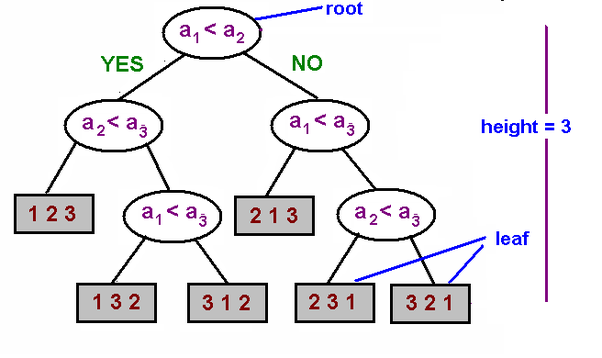
\includegraphics[width=\textwidth]{img/decision-tree.png}
    \caption{Albero delle decisioni per l'array $A[1,2,3]$}
\end{figure}

\paragraph{Osservazione} 
$$ \text{Altezza dell'albero di decisione} = \text{limite inferiore per caso pessimo}$$
\begin{align*}
    \text{per }& \text{IS} \ \quad n^2 \\
    \text{per }& \text{MS} \quad n \log n
\end{align*}

\emph{In generale}, le foglie contengono \underline{tutte} le permutazioni.
$$\# foglie \geq n! \qquad (\# foglie \leq 2^h)$$
\begin{align*}
    h & \geq \log_2 n! \\
    & \geq \log_2 \left( n(n-1)(n-2) \dots \frac{n}{2}\right) \\
    & \geq \log_2 \left( \frac{n}{2}\left(\frac{n}{2}-1\right)\left(\frac{n}{2}-2\right) \dots \frac{n}{2}\right) = \\
    & = \log_2 \left( \frac{n}{2} \right)^{(\frac{n}{2})} 
        = \frac{n}{2} \left( \log_2 n - \log_22\right)
        = \frac{n}{2} (\log_2 n - 1) = \Theta (n \log n)
\end{align*}

\subsection{Ordinamento in tempo lineare}
Esistono degli algoritmi di ordinamento che, in certe condizioni e per certi input, permettono
di ordinare in tempo lineare $\Omega (n)$

\subsubsection{Counting Sort}
Assumo
\begin{itemize}[label=$-$]
    \item interi;
    \item in $[0,k]$
\end{itemize}

\begin{itemize}[label=]
    \item \texttt{Input}: $A[1\twodots n]$ con $A[j] \in [0,k] \forall j$;
    \item \texttt{Output}: $B[1\twodots n]$ permutazione ordinata di $A$;
    \item \texttt{Supporto}: $C[0\twodots k]$.
\end{itemize}

\begin{codebox}
\Procname{\proc{CountingSort}$(A,B,k)$}
\li $C[0\twodots k] \leftarrow 0$
\li \For $j \gets 1$ \To $\attrib{A}{length}$
\zi     \Then
        \Comment $C[x] = \# elem$ in $A$ con valore $x$
\li         $C[A[j]] \gets C[A[j]] + 1$ 
        \End
\li \For $i \gets 1$ \To $k$
\zi     \Then
        \Comment $C[x] = \# elem$ in $A$ con valore $\leq x$
\li            $C[i] \gets C[i-1] + C[i]$ 
        \End
\li \For $j \gets \attrib{A}{length}$ \To $1$
\li     \Then
            $B[C[A[j]]] \gets A[j]$
\li         $C[A[j]] \gets C[A[j]] - 1$
        \End
\end{codebox} 

\paragraph{Costo?} 
\begin{align*}
    C[0,k] \leftarrow 0 && \Theta(k) \\
    \text{\texttt{for j=1}} \dots && \Theta(n) \\
    \text{\texttt{for i=1}} \dots && \Theta(k) \\
    \text{\texttt{for j=A.length}} \dots && \Theta(n)
\end{align*}
$$\text{Somma } \Theta(n+k) \text{ con } k = \Theta(1) \Rightarrow \Theta(n)$$

\paragraph{Problema di memoria} Il problema di \texttt{Counting Sort} è la memoria. 
Infatti, al crescere di $k$, la memoria richiesta per allocare \texttt{C} cresce esponenzialmente.
\begin{center}
    \begin{tabular}{|l|l|}
        \hline
        Dimensione $k$ & Memoria occupata da \texttt{C[]} \\
        \hline
        1 Byte $= 8$ bit & $2^8 \text{Bytes} = 256 \text{Bytes}$ \\
        2 Bytes $= 16$ bit & $2^{16} \text{Byte} \cdot 2 \text{Bytes} = 256 \text{Megabytes}$ \\
        8 Bytes $= 64$ bit & $2^{64} \text{Byte} \cdot 8 \text{Bytes} = 512 \text{Terabytes}$ \\
        \hline
    \end{tabular}
\end{center}
\section{Lezione del 29/03/2018}

\subsection{Radix Sort}
Il \href{https://en.wikipedia.org/wiki/Radix_sort}{Radix Sort} è un algoritmo di ordinamento in tempo
lineare $O(n)$, come \texttt{Counting Sort}, che risolve i problemi di memoria di quest'ultimo.

L'idea è quella di ordinare cifra per cifra, dalla cifra meno significativa alla più significativa con un 
algoritmo \emph{stabile}\footnote{Un algoritmo di ordinamento stabile è un algoritmo che ordina e
non scambia mai due chiavi se non è necessario (e.g. due celle con la stessa chiave).}.
\begin{align*}
	\text{(iniziale)} && \text{(terza cifra)} && \text{(seconda cifra)} && \text{(prima cifra)} \\
	329 && 720 && 720 && 329 \\
	457 && 355 && 329 && 355 \\
	657 && 436 && 436 && 436 \\
	839 && 457 && 839 && 457 \\
	436 && 657 && 355 && 657 \\
	720 && 329 && 457 && 720 \\
	355 && 839 && 657 && 839 \\
\end{align*}

\texttt{Input}: \texttt{A[1$\twodots$n]} con \texttt{A[i]} di $d$ cifre e base $b$,
\texttt{A[i]}$= a_d a_{d-1}\dots a_1$.

\begin{codebox}
\Procname{\proc{RadixSort}$(A,d)$}
\li \For $j \gets 1$ \To $d$
\li \Then
		$\text{ordina $A$ rispetto alla cifra $j$}$
		\Comment $A^j[i] = a_j a_{j-1} \dots a_1$
\zi 	$\text{con}$ \proc{CountingSort}
		\Comment $A^{j-1} ordinato$
	\End
\end{codebox}

\subsubsection{Correttezza di RadixSort(A, d)}
\begin{description}
	\item[Inizializzazione] ok;
	\item[Mantenimento] Se $A^{j-1}$ è ordinato e ordino rispetto alla $j$-esima cifra con
	un algoritmo stabile, allora $A^j$ è ordinato.
	$$i < i' \Rightarrow A^j[i] \leq A^j[i']$$
	\begin{align*}
		\text{Siano } & A^j[i] = a_j a_{j-1} \dots a_1 \\
		& A^j[i'] = a'_j a'_{j-1} \dots a_1
	\end{align*}
	
	Posso distinguere due casi:
	\begin{enumerate}
		\item \begin{align*}
			a_j \neq a'_j & \Rightarrow a_j < a'_j \\
			& \Rightarrow A^j[i] < A^j[i']
		\end{align*}
		\item \begin{align*}
			a_j = a'_j & \Rightarrow A^j[i] \leq A^j[i'] \qquad \text{(stabilità)}\\
			& \Rightarrow A^j[i] = a_j A^j[i] \leq \\
			& \leq A^j[i'] = a'_j A^{j-1}[i']
		\end{align*}
	\end{enumerate}
\end{description}

\paragraph{Costo?} 
\begin{gather*}
	d \text{ volte \texttt{CountingSort} } \; \Theta(n+b) \Rightarrow \Theta\big(d(n+b)\big) = \Theta(n) \\
	\text{con } d = \Theta(1), \text{ base } b = \Theta(n) 
\end{gather*}

\subsection{Strutture dati elementari}
\begin{itemize}[noitemsep]
	\item \emph{Tabelle hash}
	\item \emph{Alberi di ricerca}
\end{itemize}
Entrambe le strutture dati sono \emph{insiemi dinamici}: per un dato $x$, abbiamo:
\begin{itemize}[noitemsep]
	\item $x.key$;
	\item $Insert(x)$;
	\item $Delete(x)$;
	\item $Search(x)$.
\end{itemize}
\subsubsection{Tabelle Hash}
\begin{gather*}
	U \text{ universo delle chiavi} \\
	U = \{ 0, 1, \dots, \abs{U} - 1 \} \\
	T[0 \twodots \abs{U} - 1] \text{ tabella hash}	
\end{gather*}
\[ T[k] \text{ contiene} \quad
	\begin{cases}
		\text{elemento } x \text{ con } x.key = k & \text{se c'è} \\
		\bot & \text{altrimenti}
	\end{cases}
\]

\begin{codebox}
\Procname{\proc{Insert}$(T,x)$}
\li $T[\attrib{x}{\id{key}}] \gets x$
	\Comment $\Theta(1)$
\end{codebox}
\begin{codebox}
\Procname{\proc{Delete}$(T,x)$}
\li $T[\attrib{x}{\id{key}}] \gets nil$
	\Comment $\Theta(1)$
\end{codebox}
\begin{codebox}
\Procname{\proc{Search}$(k)$}
\li \Return $T[k]$
	\Comment $\Theta(1)$
\end{codebox}

\paragraph{Problema} e.g. consideriamo che la \emph{key} sia di 8 caratteri (e 8 bit per rappresentare
un carattere). Risulta molto costosa in termini di memoria la tabella hash.
\begin{gather*}
	2^8 \dots 2^8 \\
	(2^8)^8 = 2^{64} \cong 10^{19}
\end{gather*}

\paragraph{Idea} 
\begin{gather*}
	U = \{ 0, 1, \dots , \abs{U} - 1 \} \\
	T[0 \dots m-1] \qquad m << \abs{U}
\end{gather*}
La ``traduzione'' per ottenere $x.key$ da $x$ cosa comporta?
\begin{gather*}
	h : U \rightarrow \{ 0, 1, \dots , m-1 \} \text{ funzione di \emph{hashing}}\\
	n = \# elem \text{ memorizzati nella tabella } T
\end{gather*}
Se $n > m$, esisteranno $x_1, x_2 : h(x_1.key) = h(x_2.key)$.\par
\bigskip 
Abbiamo \emph{due soluzioni}:
\begin{enumerate}
	\item \textbf{Chaining} (\ref{hash:chaining});
	\item \textbf{Open Addressing} (\ref{hash:openaddessing}).
\end{enumerate}

\section{Lezione del 04/04/2018}

\subsection{Chaining}\label{hash:chaining}
Il \emph{Chaining} propone come soluzione quella di mettere sulla tabella liste dinamiche
di elementi, invece che singoli elementi, in modo che in caso si incorra in una cella
già occupata dopo un \emph{hashing}, l'elemento venga inserito in coda (o in testa) alla
lista.

\paragraph{Idea} \texttt{T[i]} $=$ lista elementi $x$ tali che $h(x.key) = i$

\begin{codebox}
\Procname{\proc{Insert}$(T,x)$}
\li	$\text{Inserisci $x$ nella lista } T[h(x.key)]$
	\Comment $O(1)$
\end{codebox}
\begin{codebox}
\Procname{\proc{Delete}$(T,x)$}
\li	$\text{Delete $x$ from } T[h(x.key)]$
	\Comment $O(1)$
\end{codebox}
\begin{codebox}
\Procname{\proc{Search}$(T,k)$}
\li	$\text{Cerca in } T[h(k)] \text{ un elemento } x \text{ tale che } \attrib{x}{\id{key}} = k$ 
	\Comment $O(n)$
\end{codebox}
\texttt{Search} ha una complessità di $O(n)$, e questo è inaccettabile.
\begin{gather*}
	n = \# \text{elementi inseriti} \\
	m = \text{dimensione di } T \\
	\alpha = \frac{n}{m} \quad \text{fattore di carico} \\
	\alpha \text{ può essere }<, \ = \text{ oppure } > \text{ di } 1
\end{gather*}

\subsubsection{Hashing uniforme semplice}
Ogni elemento di \emph{input} è ``mandato'' da $h$ con la stessa probabilità $\left( \frac{1}{m} \right)$
in una delle $m$ celle.

\paragraph{Caso medio} $\Theta(1 + \alpha)$, 1 è l'accesso alla tabella.\par
Consideriamo $n_1,n_2,\dots,n_{m-1}$ la lunghezza delle $m$ liste. La lunghezza attesa
di una lista è:
$$E[n_j] = \displaystyle\sum_{i = 1}^{n} \frac{1}{m} \cdot 1 = \frac{n}{m} = \alpha$$

\paragraph{Ricerca di una chiave} La chiave può essere:
\begin{itemize}
	\item \emph{Assente}. \texttt{Search(k)}, \texttt{k} non c'è.
	\begin{itemize}
		\item Calcolo \texttt{h(k)} $\rightarrow$ ($\Theta(1)$);
		\item Accedo a \texttt{T[h(k)] = j} $\rightarrow$ ($\Theta(1)$);
		\item Scorro $n_j$ elementi ($n_j = \alpha$) $\rightarrow (\Theta(\alpha)$).  
	\end{itemize}
	Nel complesso, ho $\Theta(1+\alpha)$

	\item \emph{Presente}. \texttt{Search(k)}, \texttt{k} presente.
	\begin{itemize}
		\item \texttt{h(k)} e \texttt{T[h(k)]}\par
			$$\text{Se } x_1, x_2,\dots x_n \text{ sono gli elementi inseriti}$$
		Costo della ricerca di $x_i$:
		\begin{align*}
			& 1 + \# elem \quad x_j : j > 1, \ h(x_i.key) = h(x_j.key) \\
			& = 1 + \displaystyle\sum_{j=i+1}^n \left(prob \ h(x_i.key) = h(x_j.key)\right) \\
			& = 1 + \displaystyle\sum_{j=i+1}^n \frac{1}{m} = 1 + \frac{n-i}{m}
		\end{align*}
		\begin{align*}
			& \frac{1}{n} \displaystyle\sum_{i=1}^n \left( 1 + \frac{n-i}{m} \right) \\
			& = \frac{1}{n} \left( n + \displaystyle\sum_{i=1}^n \frac{n-i}{m} \right) 
				= \frac{1}{n} \left( n + \frac{1}{m} \displaystyle\sum_{z=0}^{n-1} z \right) \\
			& = 1 + \frac{1}{m \cdot n} \cdot \frac{n(n-1)}{2} = 1 + \frac{n}{2m} - \frac{1}{2m} \cdot \left(\frac{n}{n} \right) \\
			& \hspace{5cm} \left(\frac{n}{m} = \alpha\right) \\
			& = 1 + \frac{\alpha}{2} - \frac{\alpha}{2n} = \Theta(1+\alpha)
		\end{align*}

		\begin{gather*}
			\text{Se } n \leq c \cdot m \text{ per qualche costante positiva } c \text{ allora}\\ 
			\alpha \leq c \Rightarrow \Theta(1)
		\end{gather*}
	\end{itemize}
	\item $h : U \implies \{ 0,1,\dots,m-1 \} \Rightarrow h(x) = 0$
\end{itemize}

\subsubsection{Funzioni Hash} Una \emph{funzione hash} deve soddisfare la proprietà di
\emph{hashing uniforme}, ossia 
\begin{quote}
	``Ogni chiave ha la stesso probabilità $\frac{1}{m}$ di essere mandata in una
	qualsiasi delle $m$ celle, indipendentemente dalle chiavi inserite precedentemente.''
\end{quote} 
Consideriamo:
\begin{itemize}
	\item $x \in [0,1)$ ($0 \leq x < 1$), $x$ chiave, estratta in modo indipendente dalla distribuzione
	uniforme (\underline{non realistica}).
	\item Allora $h(x) = \floor{mx}$ soddisfa la proprietà di \emph{hashing uniforme}.
\end{itemize} 

L'ipotesi di hash uniforme semplice dipende dalle probabilità con cui vengono estratti gli elementi da
inserire; probabilità che in genere non sono note.
Le funzioni hash che descriveremo assumono che le chiavi siano degli interi non negativi.

\paragraph{Metodo della divisione} 
$$U = \{ 0, 1, \twodots, \abs{\cup} - 1 \}$$
$$h(k) = k \mod n$$
\begin{itemize}
	\item $m = 2^p$ caso pessimo;
	\item $m = 2^p - 1$ caso non buono. $2^p$ cifre base.
\end{itemize}
La soluzione migliore è quella di scegliere chiavi lontane dalle potenze di 2, meglio
ancora se numeri primi.

\paragraph{Metodo della moltiplicazione}
$$k \in U$$
$$0 < A < 1 \text{ fissato}$$
$$h(k) = m(k A \mod 1) \qquad \text{Miglior } A : \frac{\sqrt{5}-1}{2}$$
\begin{align*}
	m & = 2^p \quad w = \# \text{bit parola} \\
	A & = \frac{q}{2^w} \quad 0 < q < 2 \\
	& m(k A \mod 1) \\
	& = m \left( k \frac{q}{2^w} \mod 1 \right) && (\text{\emph{shift} di $w$ bit, prendo la parte decimale} \\
	& && k a \mod 1 \text{ e la moltiplico per } m = 2^p) 
\end{align*}

\subsubsection{Hashing Universale} 
Per avere una distribuzione più uniforme delle chiavi nelle liste e non dipendente dall'input,
possiamo usare la \emph{randomizzazione}. \par
Insieme $H$ di funzioni di hash. Scelgo randomicamente da $H$. \par
Sotto certe ipotesi ottengo per \texttt{Search}:
$$\Theta(1 + \alpha)$$

\paragraph{Def (Hashing universale)} $\forall k_1,k_2 \in U \ k_1 \neq k_2$
\begin{gather*}
	\left| \left\{ h \in H : h(k_1) = h(k_2) \right\} \right| \leq \frac{|H|}{m} \\
	\frac{\left| \left\{ h \in H : h(k_1) = h(k_2) \right\} \right|}{|H|} \leq \frac{1}{m}
\end{gather*}

Con il \emph{chaining}, $H$ è universale per ogni $k \in U, \ j = h(k)$
\[ \text{Costo medio } \Theta(1+\alpha)
	\begin{cases}
		k \text{ non è in } T \rightarrow E[n_j] \leq \alpha \\
		k \text{ è in } T \rightarrow E[n_j] \leq 1 + \alpha
	\end{cases}
\]

\subsection{Open Addressing} \label{hash:openaddessing}

$h(k,i)$: $k$ è la chiave, $i$ è il tentativo.\par
Provo con $h(k,0)$: se capito in una cella occupata, provo con $h(k,1)$, poi $h(k,2)$
e così via, fino a che non trovo una cella libera.

Per esplorare tutta la tabella:
$$h(k,0), h(k,1), \dots, h(k,m-1)$$
che è una permutazione di 
$$0,1,\dots,m-1$$

\begin{codebox}
\Procname{\proc{Insert}$(T,x)$}
\li $i \gets 0$
\li \Repeat
\li     $j \gets h(\attrib{x}{\id{key}},i)$
\li     \If $(T[j] = \const{nil}) \kw{ or } (T[j] = \const{deleted})$ 
        \Comment posizione libera
\li         \Then
                $T[j] \gets x$
\li             \Return $j$
            \End
\li     $i \gets i + 1$
\li \Until $i = m$
\li \kw{error}
\end{codebox}
\begin{codebox}
\Procname{$\proc{Search}(T,k)$}
\li $i \gets 0$
\li \Repeat 
\li     $j \gets h(k,i)$
\li     \If $\attrib{T[j]}{key} = k$
\li     \Then
            \Return $j$
        \End
\li     $i \gets i + 1$
\li \Until $(i = m)$ \Or $(T[j] = \const{nil})$
\li \Return \const{not found}
\end{codebox} 

% 05/04/2018
\section{Lezione del 05/04/2018}

\subsection{Open Addressing} \label{hash:openaddessing}

$h(k,i)$: $k$ è la chiave, $i$ è il tentativo.\par
Provo con $h(k,0)$: se capito in una cella occupata, provo con $h(k,1)$, poi $h(k,2)$
e così via, fino a che non trovo una cella libera.

Per esplorare tutta la tabella:
$$h(k,0), h(k,1), \dots, h(k,m-1)$$
che è una permutazione di 
$$0,1,\dots,m-1$$

\begin{codebox}
\Procname{\proc{Insert}$(T,x)$}
\li $i \gets 0$
\li \Repeat
\li     $j \gets h(\attrib{x}{\id{key}},i)$
\li     \If $(T[j] = \const{nil}) \kw{ or } (T[j] = \const{deleted})$ 
        \Comment posizione libera
\li         \Then
                $T[j] \gets x$
\li             \Return $j$
            \End
\li     $i \gets i + 1$
\li \Until $i = m$
\li \kw{error}
\end{codebox}
\begin{codebox}
\Procname{$\proc{Search}(T,k)$}
\li $i \gets 0$
\li \Repeat 
\li     $j \gets h(k,i)$
\li     \If $\attrib{T[j]}{key} = k$
\li     \Then
            \Return $j$
        \End
\li     $i \gets i + 1$
\li \Until $(i = m)$ \Or $(T[j] = \const{nil})$
\li \Return \const{not found}
\end{codebox}
\begin{codebox}
\Procname{$\proc{Delete}(T,j)$}
\li $T[j] = \const{deleted}$
\end{codebox}
L'\emph{Open Addressing} risulta una soluzione inefficiente in caso
avvengano molte cancellazioni.

\subsubsection{Hashing uniforme}

Per ogni elemento di input, tutte ($m!$) le sequenze di ispezione
sono equiprobabili.

\subsubsection{Funzioni di Hash}
\begin{enumerate}
    \item \textbf{Ispezione lineare}. Sia $h'(x)$ funzione di hash ``ordinaria''. Se 
        ricado in una cella occupata, mi sposto su quella immediatamente successiva.
        $$h(k,i) = (h'(k)+i) \mod m$$
        Caratteristiche:
        \begin{itemize}
            \item è semplice;
            \item poche permutazioni ($m$ dipende solo da $h'(k)$);
            \item causa addensamenti di celle occupate (\emph{addensamento primario}).
        \end{itemize}
    \item \textbf{Ispezione quadratica}. Fisso $h'(k)$.
    $$h(k,i) = h'(k) + c_1i + c_2i^2 \qquad c_2 \neq 0$$

    \begin{codebox}
        \Procname{Inserimento di $k$}
        \zi $j \gets h'(k)$
        \zi $i \gets 0$
        \zi \While $(i < m)$ \kw{and} $(T[j] \neq \const{nil}/\const{deleted})$
        \zi \Do
                $i \gets i + 1$
        \zi     $j \gets (j + 1) \mod n$
            \End
    \end{codebox}

    \begin{description}
        \item[$(i=0) \quad$] $j = h'(k)$
        \item[$(i=1) \quad$] $j = (h'(k)+1) /mod m$
        \item[$\vdots$] 
        \item[$(i=l) \quad$] 
        \begin{align*}
            j & = \left( h'(k) + \displaystyle\sum_{i=1}^{l}i \right) \mod m \\
            & = \left( h'(k) + \frac{l(l+1)}{2} \right) \mod m \\
            & = \left( h'(k) + \frac{1}{2}l + \frac{1}{2}l^2 \right) \mod m \\
            & m = 2^p \text{ permutazione}
        \end{align*}
    \end{description}
    \item \textbf{Doppio Hash}. Fisso $h_1(k)$, $h_2(k)$
    $$h(k,i) = (h_1(k) + i \cdot h_2(k)) \mod m$$
    \emph{Osservazioni}:
    \begin{itemize}
        \item I salti sono di dimensione $h_2(k)$ all'incrementare di $i$; 
        \item Ci sono $m^2$ sequenze di ispezione;
        \item $h_2(k)$ e $m$ primi tra loro $ \quad (MCD = 1)$;
        \item $i, i<m \quad h(k,i) = h(k,i') \Rightarrow i = i' \ \quad (\text{\emph{iniettività}})$
        $$h(k, \verb|_|) : \{ 0, \_, m-1 \} \rightarrow \{ 0,\verb|_|, m-1 \}$$
        $$\text{\emph{iniettiva}} \Rightarrow \text{\emph{biiettiva}}$$
        \begin{gather*}
            h(k,i) = h(k,i') \\
            (h_1(k) + ih_2(k)) \mod m = (h_1(k) + i'h_2(k)) \mod m \\
            ((i - i')h_2(k)) \mod m = (i h_2(k) - i'h_2(k)) \mod m = 0 \\
            (i - i') \mod m = 0 \\
            i \geq i' \quad i - i' < m \\ 
            \Rightarrow i - i' = 0 \\
            \Rightarrow i = i'
        \end{gather*}
        Scelgo $m = 2^p, \ h_2(k) = 1 + 2h_2'(k)$, $h_2'(k)$ qualunque.\par
        \emph{es.} $h_2(k) = 1 + k \mod m' \quad$ con $m' < m$
    \end{itemize}
    \end{enumerate}

\paragraph{Costo?}
Il costo della \texttt{Search} con \emph{hashing uniforme} si può riassumere come segue.
$$0 \leq \alpha = \frac{n}{m} \leq 1$$

\paragraph{Ricerca di una chiave non presente}
\begin{enumerate}[label=(\alph*)]
    \item $\frac{1}{1-\alpha} \quad$ se $\alpha < 1$
    \item $m \quad$ se $\alpha = 1$ 
\end{enumerate}

\subparagraph{Probabilità di ispezionare la i-esima cella}
\begin{center}
    \begin{tabular}{c|l}
        \textbf{cella} & \textbf{probabilità} \\
        \hline
        $i = 0$ & 1 \\
        $i = 1$ & prob. cella 0 occupata: $\frac{n}{m}$ \\
        $i = 2$ & prob. cella 1 occupata: $\frac{n}{m} \cdot \frac{n-1}{m-1}$ \\
        $\dots$ \\
        $i$ & $\frac{n}{m} \cdot \frac{n-1}{m-1} \dots \frac{n-i+1}{m-i+1} \leq \alpha \cdot \alpha \dots \alpha = \alpha^i$
    \end{tabular}
\end{center}

Valore atteso per \#celle ispezionate
$$1 + \alpha + \alpha^2 + \dots + \alpha^{i-1} + \dots + \alpha^{m-1}$$

\begin{enumerate}[label=(\alph*)]
    \item $\alpha < 1 \Rightarrow \frac{1 - \alpha^m}{1 - \alpha} \leq \frac{1}{1-\alpha}$ 
    \item $m$ 
\end{enumerate}

\paragraph{Ricerca di una chiave presente}
\begin{enumerate}[label=(\alph*)]
    \item $\frac{1}{\alpha} \log \left( \frac{1}{1-\alpha} \right) \quad \alpha < 1$
    \item $1 + \log m \quad \alpha = 1$
\end{enumerate}

Finora, ho inserito $x_0,x_1,\dots, x_i,\dots,x_n$.
\begin{gather*}
    \text{costo \texttt{Search} chiave $x_i$ presente} \\
    = \text{costo \texttt{Search} chiave $x_i$ assente} \\
    \text{in }  x_0,\dots,x_{i-1} \quad \frac{1}{1-\alpha_i}, \ \alpha_i = \frac{i}{m}
\end{gather*}

Numero medio:
\begin{align*}
    & \frac{1}{n} \displaystyle\sum_{i=0}^{n-1}\frac{1}{1-\alpha_i} 
        = \frac{1}{n} \displaystyle\sum_{i=0}^{n-1} \frac{m}{m-i} 
        = \frac{m}{n}\displaystyle\sum_{i=0}^{n-1} \frac{1}{m-i} \qquad \left(\frac{m}{n} = \frac{1}{\alpha} \right)\\
    & = \frac{1}{\alpha} \displaystyle\sum_{l=m-n+1}^{m}\frac{1}{l} \qquad (m-i \rightarrow m-n+1) 
\end{align*}

\begin{itemize}
    \item Se $\alpha < 1$ %SISTEMARE, <= di cosa?
    \begin{align*}
        & \leq \frac{1}{\alpha} \int_{n-m}^{m}\frac{1}{x} \mathrm{d}x \\ 
        & = \frac{1}{\alpha}\left( \log m - \log (m-n) \right) = \frac{1}{\alpha}\left( \log \frac{m}{m-n} \right) \\
        & = \frac{1}{\alpha} \log \frac{1}{\frac{m-n}{m}} \\ 
        & = \frac{1}{\alpha} \log \left( \frac{1}{1-\left( \frac{n}{m} \right)} \right)
            = \frac{1}{\alpha} \log \left( \frac{1}{1-\alpha } \right)
    \end{align*}

    \item Se $\alpha = 1$
    \begin{align*}
        \displaystyle\sum_{l = 1}^{m} \frac{1}{l} & = 1 + \displaystyle\sum_{l=2}^m \frac{1}{l} 
            \leq \int_1^m \frac{1}{x} \mathrm{d}x \\
        & = 1 + \left( \log m - \log 1 \right) = 1 + \log m
    \end{align*}
\end{itemize}

Confrontiamo le complessità dei due casi.

\begin{center}
    \begin{tabular}{l|l|l}
        $\alpha$ & $\frac{l}{1-\alpha}$ & $\frac{1}{\alpha} \log \left( \frac{1}{1-\alpha} \right)$ \\
        \hline
        $\alpha = 0.3$  & 1.43 & 1.19 \\
        $\alpha = 0.5$  & 2.00 & 1.39 \\
        $\alpha = 0.7$  & 3.33 & 1.72 \\
        $\alpha = 0.9$  & 10 & 2.56 \\
        $\alpha = 0.99$ & 100 & 4.65         
    \end{tabular}
\end{center}
\section{Lezione del 06/04/2018}

\subsection{Max Heap con coda dinamica}
Implementiamo un \texttt{Max Heap}, solo che è implementato con una
coda dinamica invece che con un normale array.

Ogni \emph{nodo} $x$ ha 3 campi dato:
\begin{itemize}[noitemsep]
    \item \texttt{x.left};
    \item \texttt{x.right};
    \item \texttt{x.p}.
\end{itemize}

$H$ è lo \emph{heap} ($\const{nil}$ se vuoto):
\begin{itemize}[noitemsep]
    \item \texttt{H.root};
    \item \texttt{H.size}.
\end{itemize}

Abbiamo \texttt{MaxHeapify} e \texttt{MaxHeapifyUp} invariate.

\begin{codebox}
\Procname{\proc{Insert}$(H, \id{node})$}
\li \If $\attrib{H}{size} = 0$
\li     \Then
            $\attrib{\id{node}}{p} \gets \const{nil}$
\li         $\attrib{H}{root} \gets \id{node}$
\li         $\attrib{H}{size} = 1$
\li     \Else
\li         $x \gets root$
\li         $\attrib{H}{size} \gets \attrib{H}{size} + 1$
\li         $p \gets \proc{bitvector}(\attrib{H}{size})$
            \Comment $p$ letto come vettore di bit
\li         $k \gets \# \text{bit di p più significativo a 1}$
\li         \For $i \gets k-1$ \kw{down} \To $1$
\li             \Do 
                    \If $p[i] = 0$
\li                     \Then
                            $x \gets \attrib{x}{left}$
\li                     \Else 
\li                         $x \gets \attrib{x}{right}$
                    \End
            \End
\li         \If $p[0] = 0$
\li             \Then
                    $\attrib{x}{left} \gets \id{node}$
\li             \Else
\li                 $\attrib{x}{right} \gets \id{node}$
            \End
    \End
\li $\attrib{\id{node}}{left} \gets \attrib{\id{node}}{right} \gets \const{nil}$
\li $\proc{MaxHeapifyUp}(H, \id{node})$
\end{codebox} 

Raccolta esercizi della lezione: \ref{exs:6-4-2018}.
\section{Lezione del 26/04/2018}

\subsection{Alberi Binari di Ricerca (ABR)}
\paragraph{Definizione induttiva}
\begin{itemize}
	\item $\varnothing$ è un albero;
	\item Se $r$ è un nodo, $T_1$ e $T_2$ alberi $\Rightarrow r(T_1, T_2)$ è un albero.
\begin{center}
\begin{tikzpicture}
\Tree
[.r     
	[.$T_1$ ]
	[.$T_2$ ]		
]
\end{tikzpicture}
\end{center}
\end{itemize}

Ogni nodo $x$ ha i seguenti campi:
\begin{itemize}[noitemsep]
	\item $x.p$
	\item $x.key$
	\item $x.left$
	\item $x.right$
\end{itemize}

\paragraph{Proprietà}
$\forall r$
\begin{itemize}[label=$\rightarrow$]
	\item Per ogni nodo $y$ in $T_1 \quad y.key \leq x.key$;
	\item Per ogni nodo $y$ in $T_2 \quad y.key \geq x.key$. 
\end{itemize}

\subparagraph{Esempio} Ecco un \emph{albero binario di ricerca} d'esempio:
\begin{center}
	\begin{tikzpicture}
	\Tree
	[.7     
		[.3 
			[.1 ]
			[.6
				[.4 ] 
				\edge[blank]; \node[blank]{};
			]
		]
		[.9 
			[.8 ]		
			\edge[blank]; \node[blank]{};
		]
	]
	\end{tikzpicture}
\end{center}

\subsubsection{Visita simmetrica} La visita simmetrica (ordine infisso) visita i nodi in ordine
crescente.

\begin{codebox}
\Procname{\proc{In-Order}$(x)$}
\li \If $x \neq \const{nil}$
\li \Then
		\proc{In-Order}$(\attrib{x}{left})$
\li 	\proc{Print}$(x)$ \Comment $\Theta(1)$
\li 	\proc{In-Order}$(\attrib{x}{right})$
	\End
\end{codebox}

\paragraph{Costo?} 
\[ T(n) =
\begin{cases}
	c & n = 0 \\
	T(k) + T(n - k - 1) + d & n > 0, \ k < n
\end{cases}
\]

Stima di complessità: $T(n) = (c+d)n + c$. \par
Vediamo la dimostrazione (per induzione).

\begin{description}
	\item[$(n = 0)$] $T(n) = c = (c + d) \cdot 0 + c$
	\item[$(n \rightarrow n+1)$] $T(n) = T(k) + T(n-k) + d$. Non basta l'induzione ordinaria, usiamo 
	l'\emph{induzione completa}.
	\item[$(n > 0)$] Proprietà vera per $n' < n$
	\begin{align*}
		T(n) & = T(k) + T(n - k - 1) + d \\
		& \qquad \text{con } T(k) = (c+d)k + c \text{ e } T(n-k-1) = (c+d)(c-k-1)+c \\
		& = (c+d)(\cancel{k} + n - \cancel{k} - 1) + 2c + d \\
		& = n(c+d) - c - d + 2c + d \\
		& = n(c+d) + c - \cancel{d} + \cancel{d} \\
		& \cong \Theta(n)
	\end{align*}
\end{description}

\subsubsection{Ricerca} 
Ricerca di una chiave $k$ in un albero radicato nel nodo $x$.

\begin{itemize}
	\item Se $x$ è $\const{nil} \Rightarrow \text{restituisce } \const{nil}$;
	\item Altrimenti se $x.key = k \Rightarrow \text{restituisce } x$;
	\item Altrimenti, ricorre sul prossimo nodo.
\end{itemize}

\begin{codebox}
\Procname{\proc{Search}$(x,k)$}
\li \If $(x = \const{nil}) \kw{ or } (\attrib{x}{key} = k)$
\li \Then
		\Return $x$
\li \Else \If $k < \attrib{x}{key}$
\li 	\Return \proc{Search}$(\attrib{x}{left},k)$
\li \Else 
\li 	\Return \proc{Search}$(\attrib{x}{right},k)$
	\End
\end{codebox}

\paragraph{Costo?} Nel caso peggiore, il costo è l'altezza dell'albero $h$ ($O(h)$).

\bigskip
Vediamo una versione iterativa di \texttt{Search}.
\begin{codebox}
\Procname{\proc{Search-it}$(x,k)$}
\li \While $(x \neq \const{nil}) \kw{ or } (\attrib{x}{key} \neq k)$
\li \Do
		\If $k < \attrib{x}{key}$
\li 	\Then
			$x \gets \attrib{x}{left}$
\li 	\Else
\li			$x \gets \attrib{x}{right}$
		\End
	\End
\li \Return $x$
\end{codebox}

Procedura che restituisce il \emph{minimo} di un albero:
\begin{codebox}
\Procname{\proc{Min}$(T)$}
\li $x \gets \attrib{T}{root}$
\li \If $x = \const{nil}$
\li \Then
		\Return \const{nil}
\li \Else
\li 	\While $\attrib{x}{left} \neq nil$
\li 	\Do 
			$x \gets \attrib{x}{left}$
		\End
	\End
\li \Return $x$
\end{codebox}

Procedura che restituisce il \emph{massimo} di un albero.
\begin{codebox}
\Procname{\proc{Max}$(T)$}
\li $x \gets \attrib{T}{root}$
\li \If $x = \const{nil}$
\li \Then
		\Return \const{nil}
\li \Else
\li 	\While $\attrib{x}{right} \neq nil$
\li 	\Do 
			$x \gets \attrib{x}{right}$
		\End
	\End
\li \Return $x$
\end{codebox}

\subparagraph{Costo?} $O(h)$

\subsubsection{Successore di un nodo}
Si intende il nodo elencato dopo un nodo $x$ passato come parametro in una visita simmetrica.

Se le chiavi fossero tutte distinte, allora il \emph{successore} di $x$ 
è il minimo tra i ``nodi più grandi di $x$''.
\begin{itemize}
	\item Se $x$ ha un figlio destro, il \emph{successore} è $\proc{Min}(x)$;
	\item Altrimenti, il successore è l'antenato più vicino di cui $x$ è nel 
	sottoalbero sinistro.
\end{itemize}
\begin{codebox}
\Procname{\proc{Successor}$(x)$}
\li \If $\attrib{x}{right} \neq \const{nil}$
\li \Then 
		\Return \proc{Min}$(\attrib{x}{right})$
\li \Else
\li 	$y \gets \attrib{x}{p}$
\li 	\While $(y \neq \const{nil}) \kw{ and } (x = \attrib{y}{right})$
\li 	\Do
			$x \gets y$
\li 		$y \gets \attrib{y}{p}$
		\End
\li 	\Return $y$
	\End
\end{codebox}

\paragraph{Costo?} $O(h)$

%27/04/2018

\subsubsection{Inserimento}

\begin{codebox}
\Procname{\proc{Insert}$(T,z)$}
\li $x \gets \attrib{T}{root}$
\li $y \gets \const{nil}$
\li \While $x \neq \const{nil}$
\li \Do
        $y \gets x$
\li     \If $\attrib{z}{key} < \attrib{x}{key}$
\li     \Then
            $x \gets \attrib{x}{left}$
\li     \Else
\li         $x \gets \attrib{x}{right}$
        \End
    \End
\li $\attrib{z}{p} \gets y$
\li \If $y = \const{nil}$
\li \Then
        $\attrib{T}{root} \gets z$
\li \Else 
\li     \If $\attrib{z}{key} < \attrib{y}{key}$
\li     \Then
            $\attrib{y}{left} \gets z$
\li     \Else
\li         $\attrib{y}{right} \gets z$
        \End
    \End
\end{codebox}

\paragraph{Costo?} $O(h)$

\subsubsection{Eliminazione di un nodo}
Distingueremo 2 casi nell'algoritmo:
\begin{enumerate}[label=($\arabic*$)]
	\item $z$ ha al più un figlio;
	\item $z$ ha due figli.
\end{enumerate}
Per fare ciò, usiamo una funzione ausiliaria \texttt{Transplant}, con 
costo $O(1)$.

\begin{codebox}
\Procname{\proc{Transplant}$(T,u,v)$}
\li \If $\attrib{u}{p} = \const{nil}$
\li \Then
        $\attrib{T}{root} \gets v$
\li \Else
\li     \If $u = \attrib{\attrib{u}{p}}{left}$
\li     \Then
            $\attrib{\attrib{u}{p}}{left} \gets v$
\li     \Else
\li         $\attrib{\attrib{u}{p}}{right} \gets v$
        \End
    \End
\li \If $v \neq \const{nil}$
\li \Then
        $\attrib{v}{p} \gets \attrib{u}{p}$
    \End
\end{codebox} 

\begin{codebox}
	\Procname{\proc{Delete}$(T,z)$}
	\li \If $\attrib{z}{left} = \const{nil}$
	\li \Then
			$\proc{Transplant}(T,z,\attrib{z}{right})$
	\li \Else \If $\attrib{z}{right} = \const{nil}$
	\li     $\proc{Transplant}(T,z,\attrib{z}{left})$
	\li \Else
	\li     $y \gets \proc{Min}(\attrib{z}{right})$
	\li     \If $\attrib{y}{p} \neq z$
	\li     \Then
				$\proc{Transplant}(T, y, \attrib{y}{right})$
	\li         $\attrib{y}{right} \gets \attrib{z}{right}$
	\li         $\attrib{\attrib{y}{right}}{p} \gets y$
	\li         $\attrib{y}{left} \gets \attrib{z}{left}$
	\li         $\attrib{\attrib{y}{left}}{p} \gets y$
	\li         $\proc{Transplant}(T,z,y)$
	\li     \Else
	\li         $\attrib{y}{left} \gets \attrib{z}{left}$
	\li         $\attrib{\attrib{y}{left}}{p} \gets y$
	\li         $\proc{Transplant}(T,z,y)$
			\End
		\End
\end{codebox}
È possibile scrivere \texttt{Delete} in modo più compatto.

\begin{codebox}
\Procname{\proc{Delete}$(T,z)$}
\li \If $\attrib{z}{left} = \const{nil}$
\li \Then
        $\proc{Transplant}(T,z,\attrib{z}{right})$
\li \Else \If $\attrib{z}{right} = \const{nil}$
\li     $\proc{Transplant}(T,z,\attrib{z}{left})$
\li \Else
\li     $y \gets \proc{Min}(\attrib{z}{right})$
\li     \If $\attrib{y}{p} \neq z$
\li     \Then
            $\proc{Transplant}(T, y, \attrib{y}{right})$
\li         $\attrib{y}{right} \gets \attrib{z}{right}$
\li         $\attrib{\attrib{y}{right}}{p} \gets y$
        \End
\li     $\attrib{y}{left} \gets \attrib{z}{left}$
\li     $\attrib{\attrib{y}{left}}{p} \gets y$
\li     $\proc{Transplant}(T,z,y)$
    \End
\end{codebox}
\section{Lezione del 27/04/2018}

\subsection{Red-Black Trees}

I \emph{Red-Black Trees} sono ABR i cui nodi hanno un campo \emph{colore} $x.col$, che può essere:
\begin{itemize}[noitemsep]
    \item \textbf{R} per il rosso;
    \item \textbf{B} per il nero.
\end{itemize}

\paragraph{Accorgimento} $\const{nil}$ sarà in realtà un nodo,
$T.nil$, con $T.nil.col = B$.

\paragraph{Caratteristiche} \emph{RB-tree} è in realtà un ABR tale che:
\begin{enumerate}[label=($\arabic*$)]
    \item Ogni nodo $x$ ha $x.col \in \{R,B\}$; \label{rbtree:1}
    \item La radice $root$ ha $root.col = B$; \label{rbtree:2}
    \item Le foglie ($T.nil$) sono $B$; \label{rbtree:3}
    \item Se $x$ è $R$, i figli sono $B$; \label{rbtree:4}
    \item Per ogni nodo $x$, ogni cammino da $x$ a una qualsiasi delle foglie
    ha lo stesso numero di nodi $B$ (calcolato con $bh(x)$). \label{rbtree:5}
\end{enumerate} 

\begin{figure}[hbt]
    \centering
    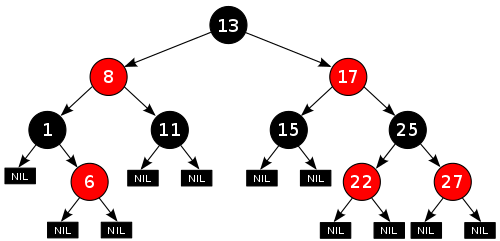
\includegraphics[width=\textwidth]{img/rb-tree-ex.png}
    \caption{Esempio di un RB-tree.}
\end{figure}
\pagebreak

È possibile notare che: 
\begin{itemize}
    \item In caso non ci fossero nodi rossi, avremo un albero
    perfettamente bilanciato;
    \item In ogni cammino, il \verb|#| di nodi \textbf{B} è almeno la
    metà del \verb|#| dei nodi \textbf{R}
\end{itemize}

\paragraph{Osservazione} Se $T$ è un \emph{RB-tree} con $n$ nodi interni ($\neq \const{nil}$)
e $h$ altezza, allora vale
$$h \leq 2 \log (n + 1)$$

\subparagraph{Dimostrazione} Consideriamo 
$$n_x \geq 2^{bh(x)} - 1$$
La dimostrazione è per induzione su $h_x$ (altezza del sotto-albero radicato in $x$).

\begin{description}
    \item[$(h_x = 1)$] Allora ho solo 
    $T.nil \Rightarrow n_x = 0 = 2^0 - 1 \qquad (2^0 \text{ con } 0 = bh(x))$
    \item[$(h_x > 1)$] Consideriamo $x$ radice. $x$ ha due figli, $x_1$ e $x_2$.\par
    Sicuramente vale $h_1,h_2 < h$. Per ipotesi induttiva, valgono:
    $$n_{x_1} \geq 2^{bh(x_1)} - 1$$
    $$n_{x_2} \geq 2^{bh(x_2)} - 1$$
    \begin{align*}
        n_x & = n_{x_1} + n_{x_2} + 1 \\
        & \geq 2^{bh(x_1)} + 2^{bh(x_2)} - 1 \\
        & \geq 2 \cdot 2^{bh(x)-1} - 1 = 2^{bh(x)} - 1 \\
        & \qquad (\text{valgono } bh(x_1) \geq bh(x)-1, \ bh(x_2) \geq bh(x)-1) \\
        \text{Comples}&\text{sivamente}\\
        n & = n_{root} \geq 2^{bh(root)} - 1
    \end{align*}
    Essendo $bh(root) \geq \frac{h}{2}$, posso ottenere
    \begin{align*}
        n_{root} & \geq 2^{bh(root)} - 1 \\
        & 2^{\frac{h}{2}} - 1 \\
        \Rightarrow \ & 2^{\frac{h}{2}} \leq n + 1 \\
        & \frac{h}{2} \leq \log_2(n+1) \Rightarrow h \leq 2 \log_2(n+1) 
    \end{align*}
\end{description}

\subsubsection{Complessità algoritmi RB-Trees}
\texttt{Search, Succ, Min, Pred, Max} hanno un costo di $O(h) = O(\log n)$

%2/5/2018

\subsubsection{RB-Insert e RB-Delete}
A differenza di quelle citate precedentemente, che risultano semplici
sia come complessità asintotica che come implementazione, Bisogna porre 
particolare attenzione a queste due procedure: \texttt{RB-Insert} e \texttt{RB-Delete}.

Per ovviare a ciò, posso utilizzare le \emph{rotazioni}. Consideriamo il seguente albero,
in cui $x$ e $y$ sono nodi normali, mentre $\alpha, \ \beta$ e $\gamma$ sono sotto-alberi
(il colore dei nodi non ha importanza ai fini della procedura che andremo a 
vedere)\footnote{Di conseguenza, applicandola a un \emph{RB-tree}, gli assiomi di validità potrebbero venire violati.}:
\begin{center}
	\begin{tikzpicture}
	\Tree
	[.$x$     
		[.$\alpha$
		]
		[.$y$ 
            [.$\beta$ 
                \edge[blank]; \node[blank]{};
                \edge[blank]; \node[blank]{};
            ]
			[.$\gamma$ 
                \edge[blank]; \node[blank]{};
                \edge[blank]; \node[blank]{};
            ]
		]
	]
	\end{tikzpicture}
\end{center}
Applichiamo la procedura \texttt{Left(T,x)}, ottenendo:
\begin{center}
	\begin{tikzpicture}
	\Tree
	[.$y$
        [.$x$
            [.$\alpha$ 
                \edge[blank]; \node[blank]{};
                \edge[blank]; \node[blank]{};
            ]
            [.$\beta$ 
                \edge[blank]; \node[blank]{};
                \edge[blank]; \node[blank]{};
            ]
		]
		[.$\gamma$ ]
	]
	\end{tikzpicture}
\end{center}

\paragraph{Osservazione} La \emph{visita simmetrica} è identica per i due alberi:
$$\alpha \rightarrow x \rightarrow \beta \rightarrow y \rightarrow \gamma$$

\begin{codebox}
\Procname{\proc{Left}$(T,x)$}
\li $\attrib{x}{right} \gets \attrib{y}{left}$
\li $\attrib{\attrib{x}{right}}{p} \gets x$
\li $\attrib{y}{left} \gets x$
\li $\attrib{x}{p} \gets y$
\li $\proc{Transplant}(T,x,y)$
\end{codebox}

\paragraph{RB-Insert(T, z)} Voglio inserire $z$ nell'albero $T$.
L'idea è quella di porre $z.col = \const{red}$ poichè meno insidioso\footnote{Andando a modificare il numero di nodi neri, cambia l'altezza nera, e la cosa è difficile da sistemare.}.
\begin{itemize}
    \item Se violo \ref{rbtree:2} $\Rightarrow z.col = \const{black}$;
    \item Se violo \ref{rbtree:4}:
    \begin{itemize}
        \item Risolvo localmente;
        \item Sposto verso l'alto il problema.
    \end{itemize}
\end{itemize}

Abbiamo due \emph{macrocasi}. $z.p$ è figlio sinistro, oppure destro. Noi analizzeremo solo il primo: \textbf{z.p figlio sinistro}.
\begin{center}
	\begin{tikzpicture}
	\Tree
	[.$\boldsymbol{z.p.p}$
        [.$\boldsymbol{\color{red} z.p}$
            [.$\boldsymbol{\color{red} z}$
            ]
		]
		[.$y$ 
        \edge[blank]; \node[blank]{};
        \edge[blank]; \node[blank]{};
        ]
    ]
	\end{tikzpicture}
\end{center}
\clearpage
Abbiamo due possibilità per $y$\footnote{I nodi con testo in rosso sono $\const{red}$, %
quelli in grassetto sono $\const{black}$, e quelli normali possono essere sia rossi che neri.}:
\begin{enumerate}
    \item $y.col = \const{red}$. Ci è sufficiente invertire il colore di $z.p.p$ con quello dei figli.
    \begin{center}
        \begin{tikzpicture}
        \Tree
        [.$\boldsymbol{\color{red} z.p.p}$
            [.$\boldsymbol{z.p}$
                [.$\boldsymbol{\color{red} z}$
                ]
            ]
            [.$\boldsymbol{y}$ 
            \edge[blank]; \node[blank]{};
            \edge[blank]; \node[blank]{};
            ]
        ]
        \end{tikzpicture}
    \end{center}
    In questo modo, risolviamo localmente e rimandiamo il problema in alto.
    \item $y.col = \const{black}$. Possiamo distinguere due sottocasi.
    \begin{enumerate}[label=($2.\arabic*$)]
        \item $z$ figlio destro. \label{rbinsert:2.1}
        \begin{center}
            \begin{tikzpicture}
            \Tree
            [.$\boldsymbol{z.p.p}$
                [.$\boldsymbol{\color{red} z.p}$
                    \edge[blank]; \node[blank]{};
                    [.$\boldsymbol{\color{red} z}$
                    ]
                ]
                [.$\boldsymbol{y}$ 
                \edge[blank]; \node[blank]{};
                \edge[blank]; \node[blank]{};
                ]
            ]
            \end{tikzpicture}
        \end{center}
        Voglio finire nel caso \ref{rbinsert:2.2}. Applico \texttt{Left(T,z.p)}, ottenendo:
        \begin{center}
            \begin{tikzpicture}
            \Tree
            [.$\boldsymbol{z.p.p}$
                [.$\boldsymbol{\color{red} z}$
                    [.$\boldsymbol{\color{red} z.p}$ ]
                    \edge[blank]; \node[blank]{};
                ]
                [.$\boldsymbol{y}$ 
                \edge[blank]; \node[blank]{};
                \edge[blank]; \node[blank]{};
                ]
            ]
            \end{tikzpicture}
        \end{center}

        \item $z$ figlio sinistro. \label{rbinsert:2.2}
        \begin{center}
            \begin{tikzpicture}
            \Tree
            [.$\boldsymbol{z.p.p}$
                [.$\boldsymbol{\color{red} z.p}$
                    [.$\boldsymbol{\color{red} z}$ ]
                    \edge[blank]; \node[blank]{};
                ]
                [.$\boldsymbol{y}$ 
                \edge[blank]; \node[blank]{};
                \edge[blank]; \node[blank]{};
                ]
            ]
            \end{tikzpicture}
        \end{center}
        Scambio i colori di $x.p.p$ con $z.p$, ottenendo:
        \begin{center}
            \begin{tikzpicture}
            \Tree
            [.$\boldsymbol{\color{red} z.p.p}$
                [.$\boldsymbol{z.p}$
                    [.$\boldsymbol{\color{red} z}$ ]
                    \edge[blank]; \node[blank]{};
                ]
                [.$\boldsymbol{y}$ 
                \edge[blank]; \node[blank]{};
                \edge[blank]; \node[blank]{};
                ]
            ]
            \end{tikzpicture}
        \end{center}
        Applico \texttt{Right(T,z.p.p)}\footnote{Analoga di \texttt{Left}.}:
        \begin{center}
            \begin{tikzpicture}
            \Tree
            [.$\boldsymbol{z.p}$
                [.$\boldsymbol{\color{red} z}$ 
                    \edge[blank]; \node[blank]{};
                    \edge[blank]; \node[blank]{};
                ]
                [.$\boldsymbol{\color{red} z.p.p}$ 
                    \edge[blank]; \node[blank]{};
                    [.$\boldsymbol{y}$ ]
                ]
            ]
            \end{tikzpicture}
        \end{center}
    \end{enumerate}
\end{enumerate}

\begin{codebox}
\Procname{\proc{RB-Insert}$(T,z)$}
\li $\proc{Insert}(T,z)$
\li $\attrib{z}{col} \gets \const{red}$
\li $\proc{RB-InsertFix}(T,z)$
\end{codebox}
\begin{codebox}
\Procname{\proc{RB-InsertFix}$(T,z)$}
\li \While $\attrib{\attrib{z}{p}}{col} = \const{red}$
\li \Do
        \If $\attrib{z}{p} = \attrib{\attrib{\attrib{z}{p}}{p}}{left}$
        \Comment Macrocaso $z.p$ figlio sinistro
\li     \Then
            $y \gets \attrib{\attrib{\attrib{z}{p}}{p}}{right}$
\li         \If $\attrib{y}{col} = \const{red}$ \Comment Caso 1
\li         \Then
                $\attrib{\attrib{\attrib{z}{p}}{p}}{col} \gets \const{red}$
\li             $\attrib{\attrib{z}{p}}{col} \gets \const{black}$
\li             $\attrib{y}{col} \gets \const{black}$
\li             $z \gets \attrib{\attrib{z}{p}}{p}$
\li         \Else \Comment Caso 2
\li             \If $z = \attrib{\attrib{z}{p}}{right}$ \Comment Caso \ref{rbinsert:2.1}
\li             \Then
                    $\proc{Left}(T,\attrib{z}{p})$
\li                 $z \gets \attrib{z}{left}$
                \End
\zi             \Comment Caso \ref{rbinsert:2.2}
\li             $\attrib{\attrib{z}{p}}{col} \gets \const{black}$
\li             $\attrib{\attrib{\attrib{z}{p}}{p}}{col} \gets \const{red}$
\li             $\proc{Right}(T,\attrib{\attrib{z}{p}}{p})$
            \End
\li     \Else $\dots$ \Comment Macrocaso $z.p$ figlio destro
        \End
    \End
\li $\attrib{\attrib{T}{root}}{col} \gets \const{black}$
\end{codebox}

\subparagraph{Costo}
$$\frac{h}{2} \cong \frac{\log n}{2} \approx \log n \text{ iterazioni senza rotazioni}
    + \proc{Max} \text{ 2 rotazioni.}$$

\paragraph{RB-Delete(T, z)}
La \texttt{Delete} è ancora più problematica\footnote{Ho deciso di ometterla per non saper come rappresentarla in modo adeguato.%
Darò solo una breve osservazione}. Se $z$ è rosso, non ho nessun problema, poichè l'altezza nera non viene toccata.
Altrimenti, i problemi possono essere diversi (radice rossa, due nodi rossi adiacenti, altezza nera inconsistente, ecc\dots).

\appendix
\appendixpage
\addappheadtotoc 

\section{Raccolta algoritmi}

\subsection{Insertion Sort}
Per approfondire, vedi la sezione \ref{insertionsort} 
\begin{codebox}
\Procname{$\proc{Insertion-Sort}(A)$}
\li $n \gets \attrib{A}{length}$
\li \For $j \gets 2$ \To $n$
		\Comment il primo elemento è già ordinato
\li	\Do
		$\id{key} \gets A[j]$ 
			\Comment $A[1 \twodots j-1]$ ordinato
\li		$i \gets j-1$
\li		\While $(i > 0)$ \And $(A[i] > \id{key})$
\li		\Do
			$A[i+1] \gets A[i]$
\li			$i \gets i-1$
		\End
\li		$A[i+1] \gets \id{key}$
	\End
\end{codebox}

\subsection{Merge Sort}
Vedi la sezione \ref{mergesort}
\begin{codebox}
\Procname{$\proc{Merge-Sort}(A,p,r)$}
\li \If $p < r$
\li \Then
        $q \gets \floor{\frac{p+r}{2}}$ 
       		\Comment arrotondato per difetto
\li     $\proc{Merge-Sort}(A,p,q)$
       		\Comment ordina \texttt{A[p$\twodots$q]}
\li     $\proc{Merge-Sort}(A,q+1,r)$
       		\Comment ordina \texttt{A[q+1$\twodots$r]}
\li     $\proc{Merge}(A,p,q,r)$
       		\Comment ``Merge'' dei due sotto-array 
    \End
\end{codebox}
\begin{codebox}
\Procname{\proc{Merge}$(A,p,q,r)$}
\li $\id{n1} \gets q-p+1$
    \Comment gli indici partono da 1
\li $\id{n2} \gets r-q$
\zi \Comment \kw{L} sotto-array sx, \kw{R} sotto-array dx
\li \For $i \gets 1$ \To $\id{n1}$
\li     \Do
            $L[i] \gets A[p+i-1]$
        \End
\li	\For $j \gets 1$ \To $\id{n2}$
\li		\Do
			$R[j] \gets A[q+j]$
        \End
\li         $L[\id{n1}+1] \gets R[\id{n2}+1] \gets \infty$
\li         $i \gets j \gets 1$
\li         \For $k = p$ \To $r$
\li             \Do
                    \If $L[i] \leq R[j]$
\li                     \Then
                            $A[k] \gets L[i]$
\li                         $i \gets i+1$
\li                     \Else
                    \Comment \texttt{L[i]} $>$ \texttt{R[j]}
\li                            $A[k] \gets R[j]$
\li                         $j \gets j+1$
                        \End
                \End
\end{codebox}

\subsection{Insertion Sort ricorsivo}

\begin{codebox}
\Procname{\proc{InsertionSort}$(A,j)$}
\li \If $j > 1$
\li     \Then
		$\proc{InsertionSort}(A,j-1)$
        \Comment ordina \texttt{A[1$\twodots$j-1]}
\li         $\proc{Insert}(A,j)$
        \Comment inserisce \texttt{A[j]} in modo ordinato in \texttt{A}
        \End
\end{codebox}
\begin{codebox}
\Procname{\proc{Insert}$(A,j)$}
\zi	\Comment Precondizione: \texttt{A[1$\twodots$j-1]} è ordinato
\li	\If $(j > 1) \ \kw{and} \ (A[j] < A[j-1])$
\li		\Then
			$A[j] \leftrightarrow A[j-1]$
		\Comment scambia le celle \texttt{j} e \texttt{j-1}
\zi		\Comment se le celle sono state scambiate, ordina 
\zi		\Comment il nuovo sottoarray \texttt{A[1$\twodots$j-1]}
\li			$\proc{Insert}(A,j-1)$
		\End
\end{codebox}

\subsubsection{Correttezza di InsertionSort(A, j)}
Procediamo per induzione:
\begin{itemize}
	\item[] $(j \leq 1) \quad$ Caso base. Array già ordinato, non faccio nulla $\Rightarrow$ ok;
	\item[] $(j > 1) \quad$ Per ipotesi induttiva, la chiamata \texttt{Insertion-Sort(A,j-1)}
	ordina \texttt{A[1$\twodots$j-1]}. Assumendo la correttezza di \texttt{Insert(A,j-1)}, esso
	``inserisce'' \texttt{A[j]} $\Rightarrow$ produce \texttt{A[1$\twodots$j]} ordinato.
\end{itemize}

\subsubsection{Correttezza di Insert(A, j)}
Anche qui, dimostrazione per induzione:
\begin{itemize}
	\item[] $(j = 1) \quad$ Caso base. \texttt{A[1]} da inserire nell'array vuoto. Non fa nulla
	$\Rightarrow$ ok;
	\item[] $(j > 1) \quad$ Due sottocasi:
	\begin{itemize}
		\item \texttt{A[j]} $\geq$ \texttt{A[j-1]}: non faccio nulla, \texttt{A[1$\twodots$j]} già
		ordinato;
		\item \texttt{A[j]} $<$ \texttt{A[j-1]}: scambio le chiavi delle due celle. Il nuovo \texttt{A[j]}
		sarà sicuramente maggiore di qualsiasi altro elemento che lo precede, poiché, per precondizione di 
		\texttt{Insert}, \texttt{A[1$\twodots$j-1]} era ordinato, e dato che valeva \texttt{A[j-1]} $\geq$ 
		\texttt{A[j]}, il nuovo \texttt{A[j]} (che è il precedente \texttt{A[j-1]}) sarà sicuramente l'elemento con il valore più alto. 
		Dopodichè, chiamo \texttt{Insert(A,j-1)} per ordinare la cella \texttt{A[j-1]}.
 	\end{itemize}
\end{itemize}
 
\subsection{CheckDup}
Algoritmo che verifica la presenza di duplicati in \texttt{A[p$\twodots$r]} e, 
solo se non ci sono, ordina l'array.

Se \texttt{A[p$\twodots$q]} e \texttt{A[q+1$\twodots$r]} ordinati e privi di duplicati:
\begin{itemize}[noitemsep]
	\item Se \texttt{A[p$\twodots$r]} non contiene duplicati, ordina e restituisce \texttt{false};
	\item altrimenti, restituisce \texttt{true}.
\end{itemize}

\begin{codebox}
\Procname{\proc{Check-Dup}$(A,p,r)$}
\li \If $p < r$
\li     \Then
            $q \gets \floor{\frac{p + r}{2}}$ 
        \Comment arrotondato per difetto
\li         \Return $\proc{Check-Dup}(A,p,q)$
\li         \mbox{ or } $\proc{Check-Dup}(A,q+1,r)$
\li         \mbox{ or } $\proc{DMerge}(A,p,q,r)$
        \End
\end{codebox}
\begin{codebox}
    \Procname{$\proc{DMerge}(A,p,q,r)$}
    \li $\id{n1} \gets q-p+1$
        \Comment gli indici partono da 1
    \li $\id{n2} \gets r-q$
    \zi \Comment \kw{L} sotto-array sx, \kw{R} sotto-array dx
    \li \For $i \gets 1$ \To $\id{n1}$
    \li     \Do
                $L[i] \gets A[p+i-1]$
            \End
    \li	\For $j \gets 1$ \To $\id{n2}$
    \li		\Do
                $R[j] \gets A[q+j]$
            \End
    \li         $L[\id{n1}+1] \gets R[\id{n2}+1] \gets \infty$
    \li         $i \gets j \gets 1$
    \li         \While $(k \leq p) \kw{ and } (L[i] \neq R[j])$ 
    \li             \Do
                        \If $L[i] < R[j]$
    \li                     \Then
                                $A[k] \gets L[i]$
    \li                         $i \gets i+1$
    \li                     \Else
                        \Comment \texttt{L[i]} $>$ \texttt{R[j]}
    \li                            $A[k] \gets R[j]$
    \li                         $j \gets j+1$
                            \End
    \li                 $k \gets k+1$
                    \End
    \li         \Return $k \leq r$
\end{codebox}


\subsubsection{Correttezza di DMerge(A, p, q, r)}
\begin{itemize}
	\item \texttt{A[p$\twodots$k-1]} è ordinato, contiene \texttt{L[1$\twodots$i-1]}$\cup$\texttt{R[1$\twodots$j-1]};
	\item \texttt{A[p$\twodots$k-1]} $<$ \texttt{L[1$\twodots$n1]}, \texttt{R[1$\twodots$n2]}.
\end{itemize}

\subsection{SumKey}
Dato \texttt{A[i$\twodots$n]} e \texttt{key} intera, \texttt{Sum(A,key)} restituisce:
\begin{itemize}
	\item \texttt{true} se $\exists i, j \in [1,n] : key = A[i] + A[j]$;
	\item \texttt{false} altrimenti.
\end{itemize}

Vediamo una prima versione, non efficiente, dell'algoritmo. Ha complessità $O(n^2)$.
\begin{codebox}
\Procname{\proc{SumB}$(A,\id{key})$}
\li	$n \gets \attrib{A}{length}$
\li	$i \gets j \gets 1$
\li \While $(i \leq n) \kw{ and } (A[i] + A[j] \neq \id{key})$
\li 	\Do
			\If $j = n$
\li				\Then
					$i \gets i + 1$
\li				\Else
\li					$j \gets j + 1$
				\End
		\End
\li	\Return $i \leq n$				
\end{codebox}

Ecco ora una versione più efficiente, che però richiede un \texttt{sorting} preventivo, che quindi causa \emph{side effect}. Si assume un 
algoritmo di sorting con complessità $O(n \log n)$. Con questa premessa, la ricerca della coppia di valori
ha complessità $O(n)$ nel caso peggiore. Nel complesso, vale quindi:
$$O(n \log n + n) = O(n \log n)$$
\begin{codebox}
\Procname{\proc{Sum}$(A,\id{key})$}
\li	$n \gets \attrib{A}{length}$
\li	\proc{sort}$(A)$
		\Comment complessità $O(n \log n)$
\li	$i \gets 1, \ j \gets n$
\li \While $(i \leq j) \kw{ and } (A[i] + A[j] \neq \id{key})$
\li 	\Do
			\If $A[i] + A[j] < \id{key}$
\li				\Then
					$i \gets i + 1$
\li				\Else
\li					$j \gets j - 1$
				\End
		\End
\li	\Return $i \leq j$	
\end{codebox}

\subsubsection{Correttezza di Sum(A, key)}
Valgono i seguenti invarianti:
\begin{enumerate}[label=(\arabic*)]
	\item \label{sum:cond1}$\forall h \in [1, i-1], \; \forall k \in [h, n] \Rightarrow A[h] + A[k] \neq key$
	\item \label{sum:cond2}$\forall k \in [j+1,n], \; \forall h \in [1,k] \Rightarrow A[k] + A[h] \neq key$
\end{enumerate}
Supponiamo di trovarci in $A[i] + A[j] < key$
\begin{itemize}[noitemsep]
	\item[$\rightarrow$] incremento $i$;
	\item[\ref{sum:cond1}] \textbf{non} cambia;
	\item[\ref{sum:cond2}] (vogliamo dimostrare) $\forall k \in [i,n] \quad A[i] + A[k] \neq key$.\par
		Distinguiamo \underline{2 casi}.
		\begin{itemize}
			\item Siccome vale $A[k] \leq A[j]$, allora
				$$A[i] + A[k] \leq A[i] + A[j] > key$$
			\item $k \in [j+1,n]$ quindi
			$$A[i] + A[k] \neq key \text{ per (2)}$$
		\end{itemize}
		Se esco perché $i > j$, \textbf{non} c'è una soluzione poiché
		$$(1) + (2) \Rightarrow \forall h \leq k \quad A[h] + A[k] \neq key$$ 
\end{itemize}

Presetiamo ora una terza soluzione, che però richiede un costo in memoria direttamente proporzionale al valore $max$ (che chiameremo $top$)
dell'array considerato, poiché richiede di allocare un array $V$ di booleani di dimensione dipendente da $top$, in cui il valore \texttt{A[i]} corrisponde alla cella \texttt{V[A[i]]}. Assumiamo
\begin{gather*}
	A[i] \geq 0 \quad \forall i \in [i,n], \ key \leq top \\
	V[v] = \text{\texttt{true} sse } \exists i : A[i] = v 
\end{gather*}
\begin{codebox}
\Procname{\proc{SumV}$(A,\id{key})$}
\li	$V[0 \twodots \id{key}] \leftarrow \const{false}$
		\Comment $\Theta (key) = O(top) = O(1)$
\li	$i \gets 1$
\li $\id{found} \gets \const{false}$
\li \While $(i \leq n) \kw{ and } not \ \id{found}$
\li 	\Do
			\If $A[i] \leq \id{key}$
\li				\Then
					$V[A[i]] \gets \const{true}$
\li					$\id{found} \gets V[\id{key} - A[i]]$
				\End
\li 		$i \gets i + 1$
		\End
\li	\Return $\id{found}$
\end{codebox}

Complessità:
\begin{itemize}
	\item $O(n)$ se $top$ costante;
	\item $O(n \cdot key)$ altrimenti.
\end{itemize}
\newpage
\subsection{Heap Sort}
Per approfondire, vedi \ref{heapsort}. 
\begin{codebox}
\Procname{\proc{Left}$(i)$}
\zi \Comment restituisce il figlio sx del nodo $i$
\li	\Return $2*i$
\end{codebox}
\begin{codebox}
\Procname{\proc{Right}$(i)$}
\zi \Comment restituisce il figlio dx del nodo $i$
\li	\Return $2*i+1$
\end{codebox}
\begin{codebox}
\Procname{\proc{Parent}$(i)$}
\zi \Comment restituisce il genitore del nodo $i$
\li	\Return $\floor{i/2}$
\end{codebox}
\begin{codebox}
\Procname{\proc{MaxHeapify}$(A,i)$}
\li $l \gets \proc{Left}(i)$
\li $r \gets \proc{Right}(i)$
\li \If $(l \leq \attrib{A}{heapsize}) \kw{ and } (A[l] > A[i])$
\li 	\Then
			$\id{max} \gets l$
\li		\Else 
\li			$\id{max} \gets i$			
		\End
\li \If $(r \leq \attrib{A}{heapsize}) \kw{ and } (A[r] > A[max])$
\li 	\Then
			$\id{max} \gets r$
		\End
\li \If $(\id{max} \neq i)$
\li 	\Then 
			$A[i] \leftrightarrow A[\id{max}]$
\li			$\proc{MaxHeapify}(A,\id{max})$
		\End
\end{codebox}
\begin{codebox}
\Procname{\proc{BuildMaxHeap}$(A)$}
\li $\attrib{A}{heapsize} = \attrib{A}{length}$
\li \For $i \gets \floor{\attrib{A}{length}/2} \kw{ down} \To 1$
\li 	\Do
			$\proc{MaxHeapify}(A,i)$
		\End
\end{codebox}
\begin{codebox}
\Procname{\proc{HeapSort}$(A)$}
\li $\proc{BuildMaxHeap}(A)$ 
    \Comment $O(n)$
\li \For $i \gets \attrib{A}{length}$ \kw{down} \To $2$
\li     \Do
            $A[1] \leftrightarrow A[i]$
\li         $\attrib{A}{heapsize} \gets \attrib{A}{heapsize} - 1 $
\li         $\proc{MaxHeapify}(A,1)$
                \Comment $O(\log n)$
        \End
\end{codebox}

\subsection{Code con Priorità}
(Sezione \ref{codeconpriorita})
\begin{codebox}
\Procname{\proc{Max}$(A)$}
\li \If $\attrib{A}{heapsize} = 0$
\li     \Then
            \kw{error}
\li     \Else
            \Return $A[1]$
        \End
\end{codebox}
\begin{codebox}
\Procname{\proc{ExtractMax}$(A)$}
\li $\id{max} \gets A[1]$
\li $A[1] \gets A[\attrib{A}{heapsize}]$
\li $\attrib{A}{heapsize} \gets \attrib{A}{heapsize} - 1$
\li $\proc{MaxHeapify}(A,1)$
        \Comment ripristina le proprietà di \emph{MaxHeap}
\li \Return $\id{max}$
\end{codebox}
\begin{codebox}
\Procname{\proc{MaxHeapifyUp}$(A,i)$}
\li \If $(i > 1) \kw{ and } (A[i] > A[\proc{Parent}(i)])$
\li     \Then
            $A[i] \leftrightarrow A[\proc{Parent}(i)]$
\li         $\proc{MaxHeapifyUp}(A,\proc{Parent}(i))$
        \End
\end{codebox}
\begin{codebox}
\Procname{$\proc{Insert}(A,x)$}
\li $\attrib{A}{heapsize} = \attrib{A}{heapsize} + 1$
\li $A[\attrib{A}{heapsize}] \gets x$
\li $\proc{Max-Heapify-Up}(A,\attrib{A}{heapsize})$
\end{codebox}
\begin{codebox}
\Procname{$\proc{Increase-Key}(A,i,\delta)$}
\zi \Comment \emph{Precondizione}: $\delta \geq 0$
\li $A[i] \gets A[i] + \delta$
\li $\proc{Max-Heapify-Up}(A,i)$
\end{codebox}
\begin{codebox}
\Procname{$\proc{Change-Key}(A,i,\delta)$}
\li $A[i] \gets A[i] + \delta$
\li \If $\delta > 0$
\li \Then
        $\proc{Max-Heapify-Up}(A,i)$
\li \Else
    	\Comment $\delta \leq 0$
\li    	$\proc{Max-Heapify}(A,i)$
    \End
\end{codebox}
\begin{codebox}
\Procname{$\proc{Delete-Key}(A,i)$}
\li $\id{old} \gets A[i]$
\li $A[i] \gets A[\attrib{A}{heapsize}]$
\li $\attrib{A}{heapsize} \gets \attrib{A}{heapsize} - 1$
\li \If $\id{old} \leq A[i]$
\li \Then $\proc{Max-Heapify-Up}(A,i)$
\li \Else
\li		$\proc{Max-Heapify}(A,i)$
    \End
\end{codebox}
\section{Esercizi}
\subsection{Ricorrenze}

\begin{itemize}[label=$\bullet$]
	\item $T(n) = aT(n-1) + b \qquad a, b > 1$
	\begin{itemize}
		\item \emph{radice}: costo $b$;
		\item la radice ha $a$ figli di costo $b$;
		\item \dots
		\item foglie terminali $O(1)$.
	\end{itemize}
	Esplicitando il caso base della ricorrenza otteniamo:
	\[ 
		T(n) =
		\begin{cases}
			c & n = 0 \\
			aT(n-1) + b & n > 0
		\end{cases}
	\]
	\begin{align*}
		T(n) & = b + ab + a^2b + \dots + a^{n-1}b + a^nc \\
		& = b \displaystyle\sum_{j=0}^{n-1}a^j + a^nc \hspace{1cm} \text{(dimostrare per induzione)}
	\end{align*}
	\begin{description}
		\item[$(a=1)$] $T(n) = nb + c = \Theta(n)$
		\item[$(a<1)$] $T(n) = \frac{1-a^n}{1-a} \cdot b + a^n c = \Theta(1)$ \par
		$\text{(valgono } \frac{1-a^n}{1-a} \leq \frac{1}{1-a}, \; a^nc < c \text{)}$
		\item[$(a>1)$] $T(n) = \frac{a^n-1}{a-1}b + a^n c = \Theta(a^n)$
	\end{description}
\end{itemize}

\subsection{Esercizi svolti il 06/04/2018} \label{exs:6-4-2018}

\paragraph{Gap} Abbiamo un \emph{gap} se $i < n$ t.c. $A[i+1] - A[i] > 1$.

Mostrare per induzione che se $A[n] - A[1] \geq n$ allora c'è un gap.

\subparagraph{Sol.}
\begin{itemize}
	\item \underline{Base}
	\begin{itemize}
		\item $n = 1 \Rightarrow A[1] - A[1] = 0$;
		\item $n = 2 \Rightarrow A[2] - A[1] > 1$ allora 1 è un gap.
	\end{itemize}
	\item \underline{Passo induttivo} $n > 2$
		Se $A[n] - A[1] \geq n$ abbiamo due casi:
		\begin{enumerate}
			\item Se $A[n] - A[n-1] > 1$ allora $A[n-1]$ è un \emph{gap};
			\item Se $A[n] - A[n-1] \leq 1$ allora
			\begin{gather*}
				A[n-1] - A[1] = \left( A[n] - A[1] \right) - \left( A[n] - A[n-1] \right) \\
				(\text{valgono } A[n-1]-A[1] \geq n \text{ e } A[n]-A[n-1] \leq 1) \\
				A[n-1] - A[1] \geq n-1 \Rightarrow A[1\twodots n-1] \text{ contiene un \emph{gap}}
			\end{gather*}
		\end{enumerate}
\end{itemize}

\begin{codebox}
\Procname{\proc{Gap}$(A,p,r)$} 
\zi \Comment pre: $r - p > 1$
\li \If $p = r + 1$
\li     \Then \Return $p$
\li     \Else
\li         $q \gets \frac{p+r}{2}$
\li     \If $A[q] - A[p] > q - p + 1$
\li         \Then
                $\proc{Gap}(A,p,r)$
\li         \Else
\li             $\proc{Gap}(A,q+1,r)$
        \End
    \End
\end{codebox}

Valutiamo la complessità con il \emph{Master Theorem}.

$$T(n) = T\left( \frac{n}{2} \right) + \Theta(1)$$
Abbiamo $a = 1, \ b = 2$. Confronto $f(n) = \Theta(1)$ con $n^{\log_2 1} = 1$.\par
Siamo nel \emph{secondo caso} del Master Theorem, poichè le due funzioni hanno lo stesso
andamento $\Rightarrow \Theta (\log^{\log_2 1} \log n) = \Theta(\log n)$

\paragraph{Select} \texttt{Select(A, k)}, ritorna il $k$-esimo elemento 
dell'array \texttt{A} se fosse ordinato.

\subparagraph{Sol.} Ci sono diverse soluzioni al problema.

\begin{enumerate}[label=($\arabic*$)]
	\item Trasformo $A$ in un \emph{MinHeap}, ed estraggo il minimo $k$ volte.
	\begin{codebox}
	\Procname{\proc{Select}$(A,k)$}
	\li	$\proc{BuildMaxHeap}(A)$ \Comment $\Theta(n)$
	\li \For $i \gets 1$ \To $k$
	\li \Do
			$x \gets \proc{ExtractMin}(A)$ \Comment $k \cdot O(\log n)$
		\End
	\li \Return $x$
	\end{codebox}

	Complessità: $O(n + k \log n)$

	\item Soluzione alternativa.
	\begin{codebox}
		\Procname{\proc{Select}$(A,k)$}
		\li	$\proc{BuildMaxHeap}(A,k)$ \Comment $\Theta(k)$
		\li \For $i \gets k+1$ \To $n$
		\li \Do
				\If $A[i] < A[1]$ \Comment $O((n-k) \log k)$
		\li		\Then
					$A[i] \leftrightarrow A[1]$
		\li			$\proc{MaxHeapify}(A,1,k)$
				\End
			\End
		\li \Return $A[1]$
	\end{codebox}

	Complessità: $O(k + (n-k) \log k) \cong O(n \log k)$
\end{enumerate}

\paragraph{Inversioni} Quante \emph{inversioni} ci sono in $A$? Implementare un algoritmo
\emph{Divide ed Impera} con complessità $O(n \log n)$ 

\subparagraph{Def (inversione)} Una coppia di indici $i, j$ tali che $i < j$ è un \emph{inversione}
per l'array $A$ se e solo se $A[i] > A[j]$.

\subparagraph{Sol.} Possiamo distinguere tre casi:
\begin{itemize}
	\item $i,j \in [p,q]$;
	\item $i, j \in [q+1,r]$;
	\item $i \in [p,q], j \in [q+1,r]$.
\end{itemize}

La soluzione che adotteremo conterà le inversioni dei tre casi separatamente, e restituirà
la somma dei tre valori ottenuti.

\begin{multline*}
	\proc{\# Inv}(p,r) = \proc{\# Inv}(p,q) + \proc{\# Inv}(q+1,r) \\
	+ | \{ (i,j) : i \in [p,q], j \in [q+1,r], A[i] > A[j] \} |
\end{multline*}

\begin{codebox}
\Procname{\proc{Inv}$(A,p,r)$}
\zi \Comment restituisce $\verb|#| inv$ e ordina l'array $A$
\li \If $p < r$ 
\li \Then
		$q = \frac{p+r}{2}$
\li		\Return $\proc{Inv}(A,p,q) + \proc{Inv}(A,q+1,r) + \proc{MergeInv}(A,p,q,r)$
\li	\Else
\li		\Return $0$
	\End
\end{codebox}

\begin{enumerate}[label=($\alph*$)]
	\item $\proc{Inv}$ non cambia gli elementi in $A[p,q]$ e $A[q+1,r]$;
	\item Il numero di inversioni ``a cavallo'' non cambia;
	\item $i,j$ inversione $A[i] > A[j]$ \par
		$\Rightarrow (i',j) \quad i' \in [i,q]$ inversione. 
\end{enumerate}

\begin{codebox}
\Procname{\proc{MergeInv}$(A,p,q,r)$}
\li $n_1 \gets q - p + 1$
\li $n_2 \gets r - q$
\li $L[1,n_1] \gets A[p,q]$
\li $R[1,n_2] \gets A[q+1,r]$
\li $L[n_1+1] \gets R[n_2+1] \gets \infty$
\li $i \gets j \gets 1$
\li $\id{inv} \gets 0$
\li \For $k \gets p$ \To $r$
\li \Do
		\If $L[i] \leq R[j]$
\li		\Then
			$A[k] \gets L[i]$
\li 		$i \gets i + 1$
\li 	\Else
\li 		$A[k] \gets R[j]$
\li 		$j \gets j + 1$
\li 		$\id{inv} \gets \id{inv} + n_1 - i + 1$ 
		\End
	\End
\li \Return $\id{inv}$
\end{codebox}

\end{document}